\documentclass[version=last,toc=bib,toc=graduated,toc=index,toc=listof,9pt,openany]{scrbook}
\usepackage[utf8]{inputenc}
\usepackage[ngerman, english]{babel}
\usepackage[default]{sourcesanspro}

\usepackage{ifmtarg}
\usepackage{ifthen}
\usepackage{etoolbox} % \ifstrempty

\usepackage{geometry}
\geometry{%a6paper
  paperwidth=125mm,
  paperheight=168mm, 
  portrait,
  top=22mm,
  inner=22mm,
  outer=20mm,
  bottom=25mm,
  headsep=3mm,
  footskip=12mm
}

\usepackage{ragged2e} % nicer typesetting (hyphenation) for non raggedright and raggedleft
\usepackage{lscape}
\setlength{\parskip}{0pt}

\usepackage{relsize}

\clubpenalty=10000 %keine Schusterjungen
\widowpenalty=10000 
\displaywidowpenalty=10000 % keine Hurenkinder

\usepackage[]{microtype}

\usepackage{graphicx} % graphics

% search path for images
\graphicspath{{images-print/}{icons/}{extra-pages/}{wallpaper/}}
\usepackage{wrapfig}  % sponsor logos wrapped with text

\usepackage{tabu}
\usepackage{tabularx}
\usepackage{longtable}
\usepackage[table,cymk]{xcolor}
\usepackage{colortbl}

% embed PDF pages
% pdfpages must not be loaded before colortbl!
\usepackage{pdfpages}
% TikZ must not be loaded before colortbl
\usepackage{tikz}

% PDFs als Hintergrundbilder
\usepackage{multirow}
\usepackage{booktabs}
\usepackage{array}


\usepackage{refcount} % calculation of the page where the map is located

% page background
\usepackage[manualmark]{scrlayer-scrpage}
\pagestyle{scrplain}

\newcommand{\acro}[1]{{\textsmaller{#1}}} % macro for abbreviations with more than one capitalised letter


% title/metadata
\title{FOSSGIS-Konferenz 2019}
\subtitle{Programm}
\author{FOSSGIS e.V.}
\date{\today}

\clearscrheadings

% page numbers
\cfoot[\begin{small}\pagemark\end{small}]{\begin{small}\pagemark\end{small}}
\ofoot[]{}
\ifoot[]{}
\pagestyle{scrplain}

% Durchschuss erhöhen
\linespread{1.15}

% include our custom macros
% command for a new time slot
\newcommand{\talkTime}{9:99}
\newcommand{\newTimeslot}[1]{\newpage\renewcommand{\talkTime}{#1}}

% new time slot but without a pagebreak
\newcommand{\newSmallTimeslot}[1]{\renewcommand{\talkTime}{#1}}

% initialise \conferenceDay 
\newcommand{\conferenceDay}{Noday}


% define default page style (cutting marks with page number)
\DeclareNewLayer[background, oddorevenpage, width=125mm,%
height=169mm, contents={%
  
\includegraphics{wallpaper/crop-marks.pdf}%
}]{cropmarksevery}
\newpairofpagestyles[scrheadings]{cropmarksstyle}{}
\AddLayersAtBeginOfPageStyle{cropmarksstyle}{cropmarksevery}

% page style for title pages
\DeclareNewLayer[background, oddorevenpage, width=125mm,%
height=169mm, contents={%
  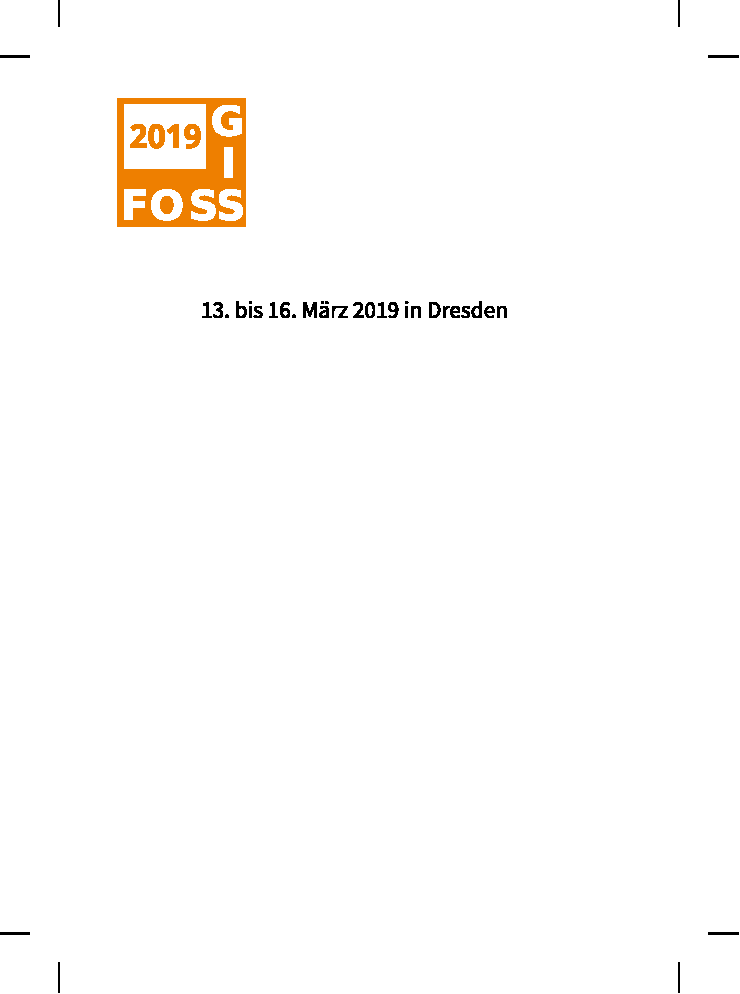
\includegraphics{wallpaper/front-cover-with-crop-marks.pdf}%
}]{titlelayer}
\newpairofpagestyles[]{titlestyle}{}
\AddLayersAtBeginOfPageStyle{titlestyle}{titlelayer}

% define alias commands for all three days
\def\mittwoch{Mittwoch}
\def\donnerstag{Donnerstag}
\def\freitag{Freitag}

% define Wednesday page style
\DeclareNewLayer[background, oddpage,  width=125mm,%
height=169mm, contents={%
  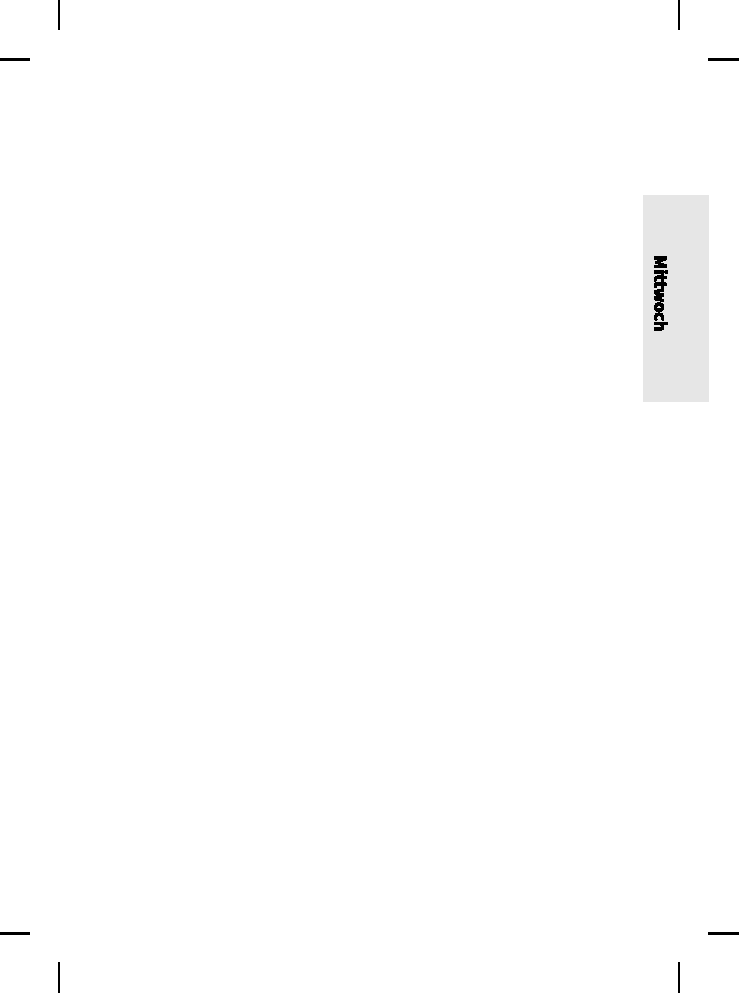
\includegraphics{wallpaper/mittwoch-ungerade.pdf}%
}]{mittwochungerade}
\DeclareNewLayer[background, evenpage,  width=125mm,%
height=169mm, contents={%
  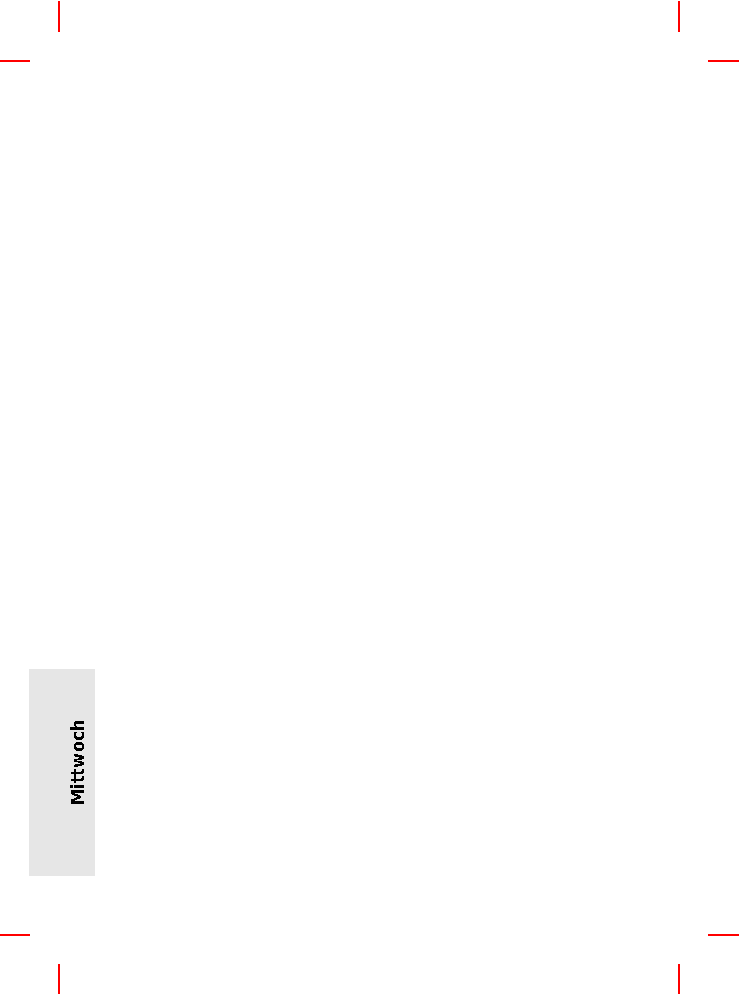
\includegraphics{wallpaper/mittwoch-gerade.pdf}%
}]{mittwochgerade}
\newpairofpagestyles[scrheadings]{mittwoch}{}
\AddLayersAtBeginOfPageStyle{mittwoch}{mittwochgerade}
\AddLayersAtBeginOfPageStyle{mittwoch}{mittwochungerade}

% define Thursday page style
\DeclareNewLayer[background, oddpage,  width=125mm,%
height=169mm, contents={%
  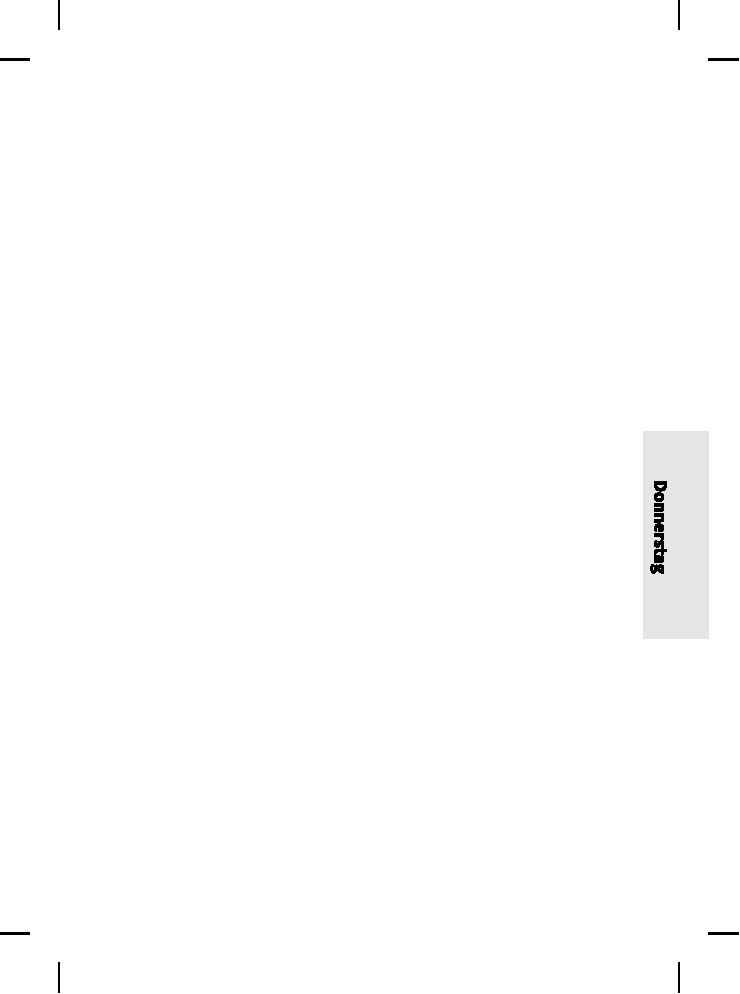
\includegraphics{wallpaper/donnerstag-ungerade.pdf}%
}]{donnerstagungerade}
\DeclareNewLayer[background, evenpage,  width=125mm,%
height=169mm, contents={%
  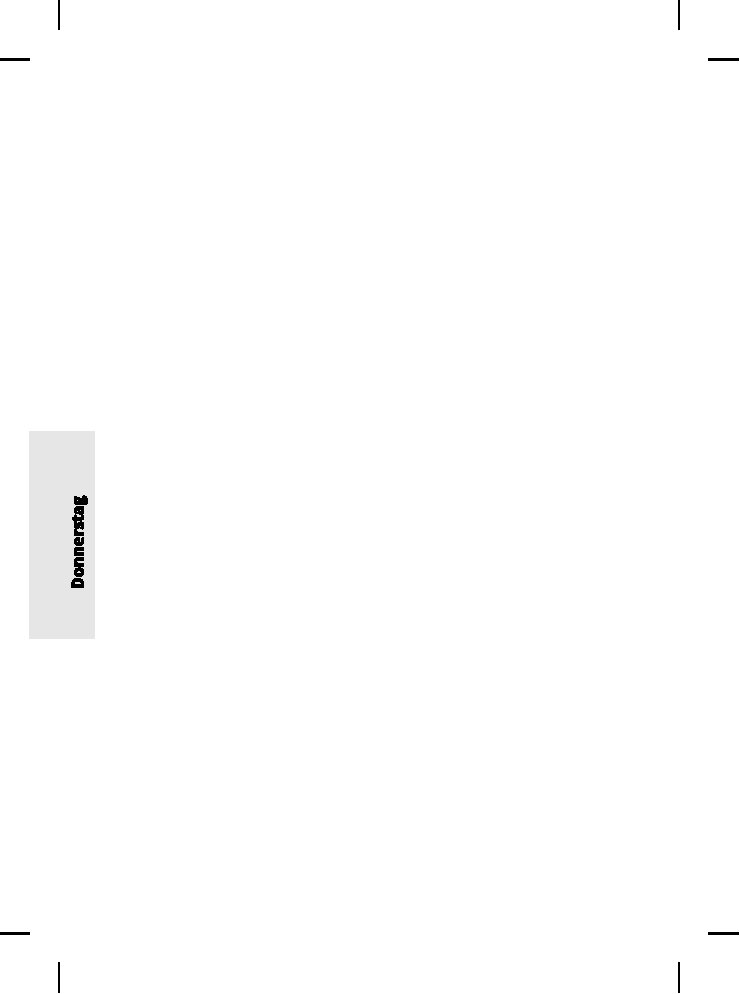
\includegraphics{wallpaper/donnerstag-gerade.pdf}%
}]{donnerstaggerade}
\DeclareNewLayer[background, oddpage,  width=125mm,%
height=169mm, contents={%
  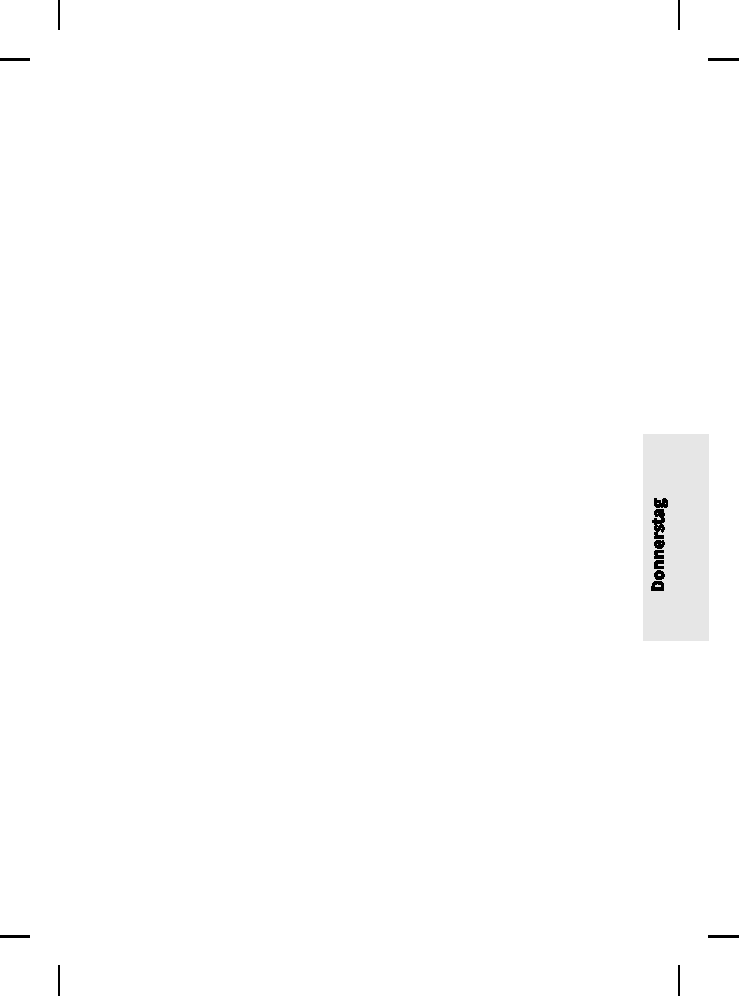
\includegraphics{wallpaper/donnerstag-ungerade-gedreht.pdf}%
}]{donnerstagungeradegedreht}
\newpairofpagestyles[scrheadings]{donnerstag-tabelle}{}
\AddLayersAtBeginOfPageStyle{donnerstag-tabelle}{donnerstaggerade}
\AddLayersAtBeginOfPageStyle{donnerstag-tabelle}{donnerstagungeradegedreht}
\newpairofpagestyles[scrheadings]{donnerstag}{}
\AddLayersAtBeginOfPageStyle{donnerstag}{donnerstaggerade}
\AddLayersAtBeginOfPageStyle{donnerstag}{donnerstagungerade}

% define Friday page style
\DeclareNewLayer[background, oddpage,  width=125mm,%
height=169mm, contents={%
  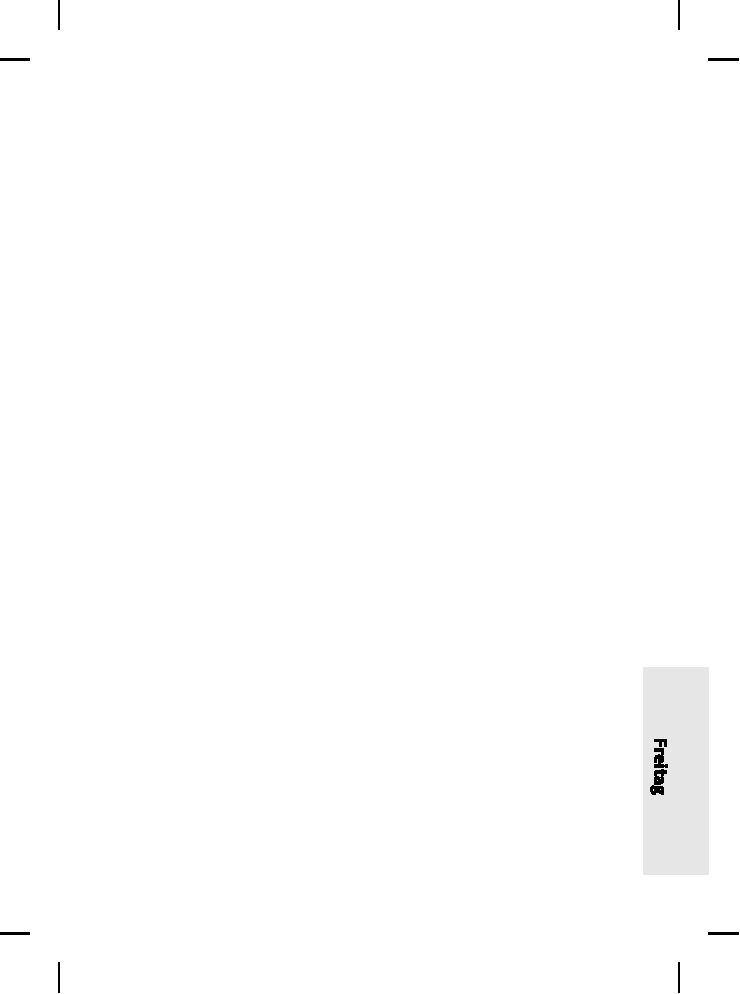
\includegraphics{wallpaper/freitag-ungerade.pdf}%
}]{freitagungerade}
\DeclareNewLayer[background, evenpage,  width=125mm,%
height=169mm, contents={%
  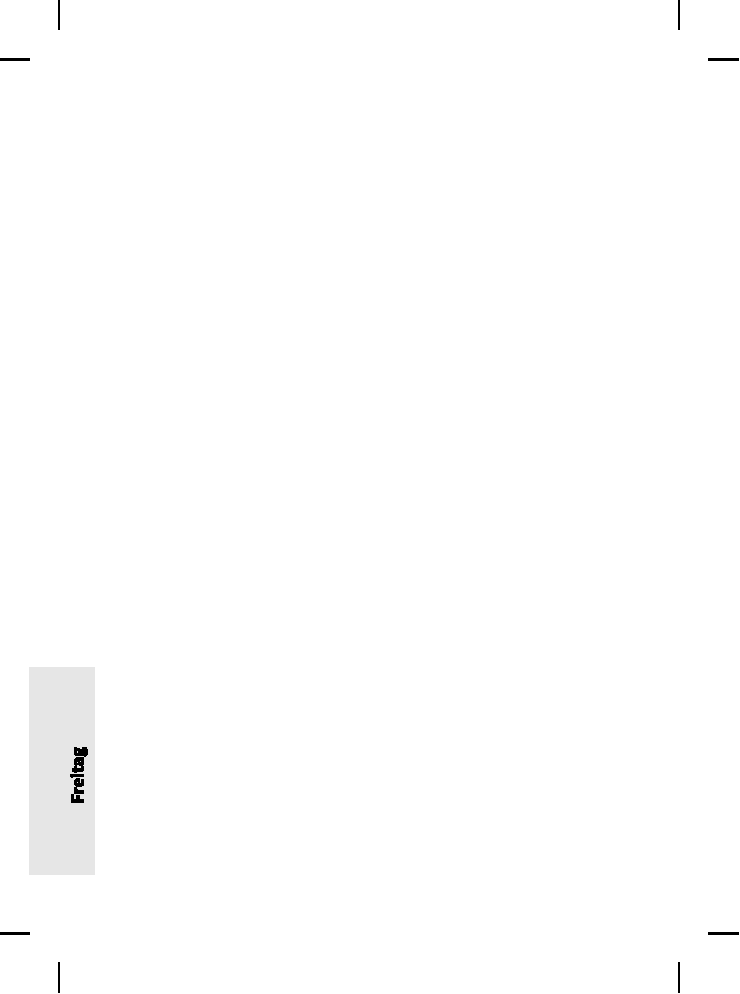
\includegraphics{wallpaper/freitag-gerade.pdf}%
}]{freitaggerade}
\DeclareNewLayer[background, oddpage,  width=125mm,%
height=169mm, contents={%
  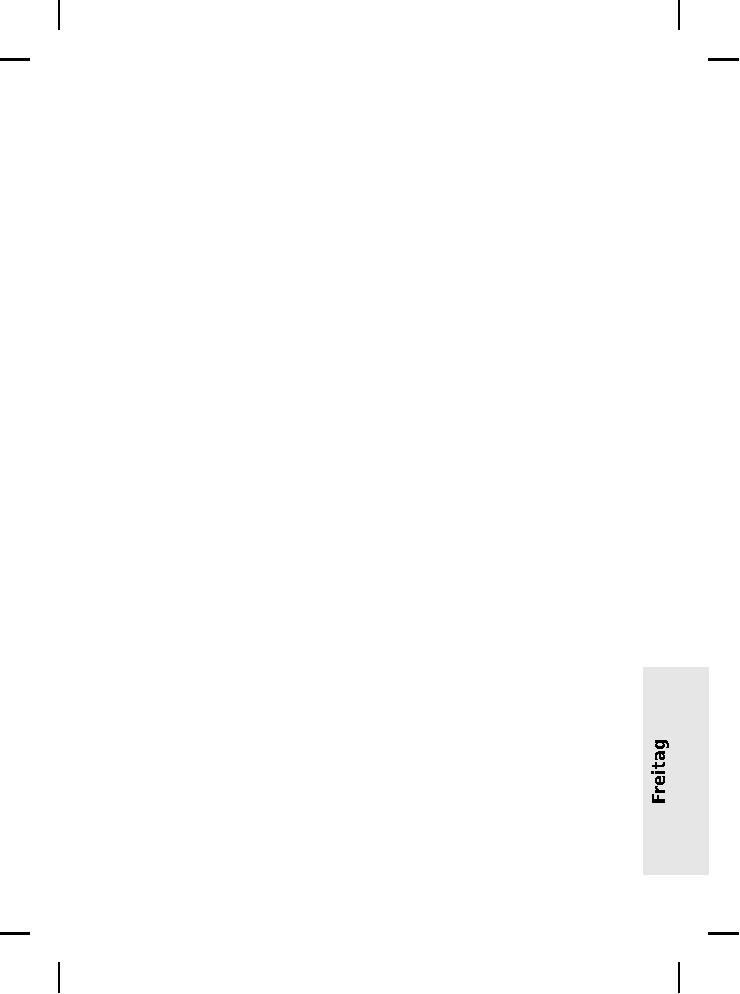
\includegraphics{wallpaper/freitag-ungerade-gedreht.pdf}%
}]{freitagungeradegedreht}
\newpairofpagestyles[scrheadings]{freitag-tabelle}{}
\AddLayersAtBeginOfPageStyle{freitag-tabelle}{freitaggerade}
\AddLayersAtBeginOfPageStyle{freitag-tabelle}{freitagungeradegedreht}
\newpairofpagestyles[scrheadings]{freitag}{}
\AddLayersAtBeginOfPageStyle{freitag}{freitaggerade}
\AddLayersAtBeginOfPageStyle{freitag}{freitagungerade}

% \setpagebackground selects the page style to be used depending on the current day. Each day has
% its own page style.
\newcommand{\setPageBackground}{ %
  \ifthenelse{\equal{\conferenceDay}{\mittwoch}}{%
    \pagestyle{mittwoch}
  }{}
  \ifthenelse{\equal{\conferenceDay}{\donnerstag}}{%
    \pagestyle{donnerstag}
  }{}
  \ifthenelse{\equal{\conferenceDay}{\freitag}}{%
    \pagestyle{freitag}
  }{}
}


% additional column type for tables
\newcolumntype{Y}[1]{>{\RaggedRight\arraybackslash}p{#1}}

%% length of the title boxes
\newlength{\titleboxwidth}
\setlength{\titleboxwidth}{\textwidth}
\advance\titleboxwidth by -6pt

% command to lay out the title boxes
\newcommand{\setAbstract}[6]{
  % 1. speaker
  % 2. title
  % 3. subtitle
  % 4. abstract (Text)
  % 5. colour
  % 6. room
  %\thispagestyle{scrheadings}
  \setPageBackground
  \setlength\tabcolsep{0pt}
  % \setlength{\fboxsep}{0pt}
  \noindent\fcolorbox{white}{#5}{%
    \parbox{\titleboxwidth}{%
      \noindent\begin{tabu}{X[5L]r}
        \isSpeakerEmpty{#1}{#2}{#6}
        \isSubtitleEmpty{#3}
      \end{tabu}%
    }%
  }%
  %
  \isAbstractEmpty{#4}%
  \vspace{0.5em}% space to the next talk even if there is no abstract
  \setlength\tabcolsep{6pt} % set column padding back to default value
}

% lay out the speaker if there is any
% We assume that there is only a subtitle if the talk has a speaker.
\makeatletter
  \newcommand{\isSpeakerEmpty}[3]{%
    % Arguments:
    % 1. speaker
    % 2. title
    % 3. room
    \@ifmtarg{#1}{%
      \par\noindent\large \sectfont #2% % titel
      &
      #3, \talkTime
      \tabularnewline
    }%
    {
      \emph{#1} % Sprecher
      &
      \talkTime
      \tabularnewline
      {%
        \par\noindent\large \sectfont #2%
      }% % titel
      &
      #3
      \tabularnewline
    }%
  }
\makeatother

% Lay out the subtitle
% has to be a separate function and has to be surrounded by \makeatletter for technical reasons
\makeatletter
  \newcommand{\isSubtitleEmpty}[1]{%
    \@ifnotmtarg{#1}{%
      \multicolumn{2}{Y{\linewidth}}{%
        \vspace{-0.6em}%
        \noindent%
        \bfseries
        \normalsize
        \sectfont #1%
      }
      \tabularnewline%
    }
  }
\makeatother

% Lay out the abstract if there is any
% has to be a separate function and has to be surrounded by \makeatletter for technical reasons
\makeatletter
\newcommand{\isAbstractEmpty}[1]{%
  \ifstrempty{#1}{%
    \vspace{1.5em}%
  }{%
    \vspace{0.5em}\newline%
    #1 \par% % abstract
    \vspace{1.5em}% space to the next talk even if there is an abstract
  }%
}
\makeatother

% define colours
%\definecolor{eins}{cmyk}{0 .18 .06 .10}
\definecolor{eins}{cmyk}{0 .13 .04 .08}
\definecolor{zwei}{cmyk}{.1 0 .17 .05}
\definecolor{hellorange}{cmyk}{0 0.18 0.40 0.03}
\definecolor{audimax}{cmyk}{0.13 0 0.04 0.11}
\definecolor{geoblau}{cmyk}{0.24 .02 0 .01}
\definecolor{dezentrot}{cmyk}{0 .24 0.29 .04}
\definecolor{hellgelb}{cmyk}{0 .02 0.36 0}
\definecolor{hellgruen}{cmyk}{0.10 .0 0.22 0.05}

% abstract at Audimax (S239)
\newcommand{\abstractAudimax}[4]%
{%
  \setAbstract{#1}{#2}{#3}{#4}{audimax}{Audimax}
}

% abstract at Mathe (Z211) 
\newcommand{\abstractMathe}[4]%
{%
  \setAbstract{#1}{#2}{#3}{#4}{hellgelb}{Mathe}
}

% abstract at Physik (Z254)
\newcommand{\abstractPhysik}[4]%
{%
  \setAbstract{#1}{#2}{#3}{#4}{hellgruen}{Physik}
}

% event at Bärenzwinger
\newcommand{\abstractBaerenzwinger}[4]%
{%
  \setAbstract{#1}{#2}{#3}{#4}{dezentrot}{Bärenzwinger}
}

% abstract at Recht (Z208)
\newcommand{\abstractRecht}[4]%
{%
  \setAbstract{#1}{#2}{#3}{#4}{geoblau}{Recht}
}

% abstract at a different location
\newcommand{\abstractOther}[5]%
{%
  \setAbstract{#1}{#2}{#3}{#4}{hellorange}{#5}
}

% infobox for workshops (they don't have an abstract in the booklet)
\newcommand{\workshopbox}[3]{%
  % 1. titel
  % 2. speaker
  % 3. Room
  \setlength\tabcolsep{0pt}
  \noindent\fcolorbox{white}{dezentrot}{%
    \parbox{\titleboxwidth}{%
      \noindent%
      \begin{tabu}{X[5L]r}
        \emph{#2} % Sprecher
        &
        \talkTime
        \tabularnewline
        {\noindent\large \bfseries #1}% % title
        &
        #3
        \tabularnewline
      \end{tabu}
    }
  }
  \setlength\tabcolsep{6pt} % set column padding back to default
}

% too long
\newcommand{\tooLong}{Dieser Text ist viel zu lang. Dieser Text ist viel zu lang. Dieser Text ist viel zu lang. Dieser Text ist viel zu lang. Dieser Text ist viel zu lang. Dieser Text ist viel zu lang. Dieser Text ist viel zu lang. Dieser Text ist viel zu lang. Dieser Text ist viel zu lang. Dieser Text ist viel zu lang. Dieser Text ist viel zu lang. Dieser Text ist viel zu lang. Dieser Text ist viel zu lang. Dieser Text ist viel zu lang. }

\newlength{\fboxwidth}

\def\workshopsSection{workshopsSection}
\def\abstractsSection{abstractsSection}

% boxes for text-only advertisement texts by our sponsors
\newcommand{\sponsorBox}[4]{%
  \setlength{\fboxwidth}{\textwidth}
  \advance\fboxwidth by -7.0pt
  \abstractSponsorbox{#1}{#2}{#3}{#4}{\workshopsSection}%
}

\newcommand{\sponsorBoxA}[4]{%
  \setlength{\fboxwidth}{\textwidth}
  \advance\fboxwidth by -10.0pt
  \abstractSponsorBox{#1}{#2}{#3}{#4}{\abstractsSection}%
}

%% box for advertisment by a sponsor
%% 1. logo
%% 2. width of the logo
%% 3. number of required lines of the logo (due to usage of wrapfigure)
%% 4. text
%% 5. Umfeld (\workshopsSection oder \abstractsSection}
\makeatletter
  \newcommand{\abstractSponsorbox}[5]{%
    \setlength{\fboxsep}{4.5pt}%
    \noindent%
    \ifthenelse{\equal{#5}{\workshopsSection}}{%
      \hspace{2.65pt}%
    }{%
      \hspace{-1pt}%
    }%
    \fcolorbox{gray}{white}{%
      \parbox{\fboxwidth}{
        \@ifmtarg{#1}{}{%
          \begin{wrapfigure}[#3]{r}[0pt]{#2}
            \centering\vspace{-1\baselineskip}
            \includegraphics[width=#2]{#1}
          \end{wrapfigure}
        }
  
        \noindent #4
      }%
    }
    \setlength{\fboxsep}{3pt}
  }
\makeatother

% definition of column types for the schedule tables
\newcolumntype{Z}[1]{>{\RaggedRight\arraybackslash}p{#1}}%
\newcolumntype{C}[1]{>{\Centering\arraybackslash}p{#1}}%

% common implementation of typesetting of a session in the tables
\newcommand{\talkInternal}[2]{%
  \textbf{#1}
  \ifthenelse{\equal{#2}{}}{}{%
    \newline\emph{#2}%
  }
}

% macro to typeset a talk in the schedule tables spanning over more than one row:
% usage: \longTalk{rowcount}{title}{speaker}
\newcommand{\longTalk}[3]{%
  &
  \multirow{#1}{\linewidth}{%
    \parbox{\linewidth}{
      %HACK Inserting a \vspace here is a dirty hack but it works.
      \vspace{0.45\baselineskip}
      \talkInternal{#2}{#3}%
    }
  }%
}%

% macro to typeset a talk in the schedule tables spanning over more than one row:
% usage: \talk{title}{speaker}
\newcommand{\talk}[2]{%
  &
  \talkInternal{#1}{#2}%
}%


\newcommand{\workshop}[3]%
{%
  \workshopbox{#1}{#2}{#3}
}%

\newcommand{\otherevent}[1]%
{%
  & \textbf{#1}
}%

\newcommand{\audimaxEvent}[2]%
{%
  &
  \multicolumn{3}{c}{
    \textbf{#1} (Audimax) \par \emph{#2}
  }
}%

\newcommand{\coffeespace}{\vspace{0.4em}}
\newcommand{\workshopspace}{\vspace{0.5em}\\}

% define colors
\definecolor{commongray}{gray}{.9}
\renewcommand{\arraystretch}{1.4}



\begin{document}
 
\pagestyle{cropmarksstyle}
\begin{titlepage}
  \thispagestyle{titlestyle}
  \null
\end{titlepage}
\pagestyle{cropmarksstyle}

\selectlanguage{ngerman}
\section*{Inhalt}

\vspace*{0.35em}%
\noindent Workshops am Mittwoch \dotfill \pageref{mittwoch-workshops}

\vspace*{0.35em}%
\noindent Workshops am Donnerstag \dotfill \pageref{donnerstag-workshops}

\vspace*{0.35em}%
\noindent Workshops am Freitag \dotfill \pageref{freitag-workshops}

\vspace*{0.35em}%
\noindent Vorträge am Mittwoch \dotfill \pageref{mittwoch}

\vspace*{0.35em}%
\noindent Vorträge am Donnerstag \dotfill \pageref{donnerstag}

\vspace*{0.35em}%
\noindent Vorträge am Freitag \dotfill \pageref{freitag}

\vspace*{0.35em}%
\noindent OSM-Samstag \dotfill \pageref{osm-samstag}

\vspace*{0.35em}%
\noindent Impressum \dotfill \pageref{impressum}

\newpage

\newpage
\section*{Willkommen zur FOSSGIS-Konferenz 2019 in Dresden!} \label{welcome}
Die Abkürzung FOSSGIS steht für freie und Open"=Source"=Software für Geoinformationssysteme.
Die FOSSGIS"=Konferenz ist im deutschsprachigen Raum die führende Konferenz zu diesem Thema
und wird dieses Jahr vom gemeinnützigen FOSSGIS e.V.
gemeinsam mit der Hochschule für Technik und Wirtschaft Dresden organisiert.

Ziel der jährlich stattfindenden Konferenz ist die Verbreitung von freier und
Open-Source-Software für Geoinformationssysteme. In den nächsten vier Tagen
haben Sie die Gelegenheit, sich mit Entwicklern und anderen Anwendern auszutauschen und
neueste Informationen zu Anwendungs- und Arbeitsmöglichkeiten zu erhalten. Im
Foyer des Geozentrums werden Firmen und Projekte ihr Knowhow präsentieren.

\newpage
\section*{Goldsponsor}
\begin{center}
	
\includegraphics[width=0.8\textwidth]{001_Wheregroup}
\end{center}
Die WhereGroup gehört in Deutschland zu den führenden Anbietern von Geoinformationssystemen mit
Open-Source-Software. Wir bieten alle Dienstleistungen rund um Beratung, Konzeption, Entwicklung,
Aufbau und Betrieb dynamischer Kartenanwendungen im Intra- und Internet. Darüber hinaus gehört ein
umfangreiches Schulungs- und Workshop-Programm zu unserem Portfolio.

Gegründet wurde das Unternehmen als eine Fusion drei verschiedener Unternehmen in Bonn. Im Jahr 2017
haben wir unser 10-jähriges Jubiläum gefeiert. Das WhereGroup-Team umfasst heute über 40 Angestellte
unterschiedlicher Fachrichtungen verteilt auf die Standorte Bonn (Hauptsitz), Freiburg und Berlin.

Das Spektrum unserer Lösungen reicht von Geoportalen und kartenbasierter Datenverwaltung bis hin zu
hochverfügbaren Anwendungen für die freie Wirtschaft und die öffentliche Verwaltung.

In unseren Projekten setzen wir auf die Standards bzw. Empfehlungen des Open Geospatial Consortiums
(OGC), der INSPIRE-Richtlinie und der GDI-DE. Ihre Verwendung gewährleistet ein Maximum an
Interoperabilität und Flexibilität unserer Lösungen. Die Einhaltung hoher Sicherheitsstandards ist
für uns nicht zuletzt durch unsere Projekte mit Landes- und Bundesbehörden sowie Großkonzernen eine
Selbstverständlichkeit.

Wir beraten absolut herstellerunabhängig und sind spezialisiert auf die professionelle Anwendung,
Weiterentwicklung und Integration offener Standards und bewährter Open-Source-Technologien und
freier Software. Dazu zählen neben unseren Projekten Mapbender, Metador und PostNAS unter anderem
GeoServer, MapServer, MapProxy, OpenLayers, PostGIS, QGIS und OpenStreetMap.

Über unser Schulungsinstitut, die FOSS Academy, bieten wir praxisorientierte Schulungen zum Thema
„GIS mit Open-Source-Software“ an. Diese können sowohl von Einzelpersonen, als auch von Firmen, auf
Wunsch auch als Inhouse-Schulungen, gebucht werden.

Die WhereGroup ist bundesweit und international mit Hochschulen, Firmen und Verbänden vernetzt. Wir
verfügen über langjährige, persönliche Kontakte zu diversen Universitäten und Hochschulen im In- und
Ausland, zum FOSSGIS e.V., zur Open Source Geospatial Foundation (OSGeo), zum Open Geospatial
Consortium (OGC), sowie zu den Herstellern bzw. Maintainern der gängigsten Open-Source-Produkte im
Geo-Bereich. Zu unserer Überzeugung gehört, dass wir uns aktiv in die Geoinformatik-Community
einbringen. Es ist uns wichtig, an der Diskussion und Weiterentwicklung von verschiedensten
Open-Source-Lösungen mitzuwirken.

Mehr zur WhereGroup unter www.wheregroup.com und www.foss-academy.com.

\section*{Goldsponsor}
\begin{center}
  
\includegraphics[width=0.7\textwidth]{002_here-xyz}
\end{center}
Über HERE: HERE ist seit 1985 Entwickler und Anbieter von heute cloudbasierten Kartendiensten und will es Menschen, Unternehmen und Städten ermöglichen vom Potenzial ortsbezogener Technologie zu profitieren. Dadurch können bessere, effizientere und nachhaltigere Ergebnisse erzielt werden – angefangen von der Navigation ans Fahrtziel über städtisches Infrastrukturmanagement bis hin zur Optimierung von Flotten und Warenströmen.

Mehr zum Unternehmen auf https://www.here.com/

HERE XYZ: Unser neuestes Produkt, HERE XYZ, ist ein Service für Kartographen, Mapping-Enthusiasten und Entwickler die einfacher mit räumlichen Daten arbeiten wollen. Als Zugriffspunkt ermöglichen HERE XYZ Komponenten den Upload, das Management, die Darstellung und das Teilen eigener und externer Daten sowohl öffentlicher oder privater mit größtmöglicher Freiheit und Flexibilität. Mit dem XYZ Hub können diese in Echtzeit bearbeitet werden, ohne gleichzeitig die Komplexität der technischen Infrastruktur lösen zu müssen.

Nutzer können weiter auf ihre bevorzugten Tools setzen oder um neue Werkzeuge zur Arbeit mit Geodaten erweitern: Das XYZ Studio bietet die Möglichkeit zur schnellen Visualisierung und Publikation von Daten. Mit dem HERE Command Line Interface (CLI) steht ein weiteres, mächtiges Tool zum Transport von Daten bereit.

\emph{Offen} und \emph{interoperabel} stellen dabei die Grundsätze dar: Alle Daten im XYZ Hub sind über die REST API mit konfigurierbaren Freigaben direkt in Standardformaten wie GeoJSON und MVT verfügbar und können somit leicht mit verschiedensten Tools verwendet, weiterverarbeitet und natürlich angezeigt werden. Weiterhin werden Kernkomponenten bald als Open Source Projekte betrieben und wir hoffen es dort mit der Community gemeinsam voranzutreiben. Alles das gibt es auf https://here.xyz/

Open Source in HERE Wie viele andere nutzen wir bei HERE natürlich auch Open Source Software und unterstützen OSS aktiv. Beispielsweise sind wir Mitglied der Linux Foundation, und der TODO Group, deren Ziel es ist die Open Source-Denkweise in Firmen zu etablieren.

HERE trägt nicht nur häufig durch Verbesserungen und Erweiterungen zu großen und kleinen Open Source Projekten bei. Sehr aktive Projekte sind auch bei uns entstanden, wie beispielsweise das OSS Review Toolkit, das wir zusammen mit vielen Partnern und Kontributoren vorantreiben, um die unterschiedlichsten Open Source Lizenzen in Software automatisch zu erkennen und zu katalogisieren. Dies erleichtert den professionellen Einsatz von OSS durch Transparenz and Lizenzanforderungen speziell in komplexen Projekten. Mehr Informationen findet ihr auf GitHub unter https://github.com/heremaps/


%
% time: Wednesday 10:30
% URL: https://pretalx.com/fossgis2019/talk/9U9E7P

\noindent\newSmallTimeslot{2019-03-13 10:30:00+01:00}
\workshop{Vektor-Tiles erstellen und publizieren}{Pirmin Kalberer}{Workshop GDV}
\workshopspace

%%%%%%%%%%%%%%%%%%%%%%%%%%%%%%%%%%%%%%%%%%%

% time: Wednesday 10:30
% URL: https://pretalx.com/fossgis2019/talk/9AWSVU

\noindent
\workshop{QGIS für Fortgeschrittene}{Stephan Herritsch, Arne Schubert}{Workshop GI}
\workshopspace

%%%%%%%%%%%%%%%%%%%%%%%%%%%%%%%%%%%%%%%%%%%

% time: Wednesday 10:30
% URL: https://pretalx.com/fossgis2019/talk/K9DD8V

\noindent
\workshop{GeoServer Vertiefung}{Daniel Koch, Marc Jansen}{Workshop LM}
\workshopspace

%%%%%%%%%%%%%%%%%%%%%%%%%%%%%%%%%%%%%%%%%%%

% time: Wednesday 15:00
% URL: https://pretalx.com/fossgis2019/talk/MC7QUJ

\noindent\newSmallTimeslot{2019-03-13 15:00:00+01:00}
\workshop{Workshop Datenschutz und geographische Informationen}{Falk Zscheile}{Recht Z208}
\workshopspace

%%%%%%%%%%%%%%%%%%%%%%%%%%%%%%%%%%%%%%%%%%%

% time: Wednesday 15:00
% URL: https://pretalx.com/fossgis2019/talk/8CPGTJ

\noindent
\workshop{Geodaten jonglieren mit ogr2ogr}{Claas Leiner}{Workshop GDV}
\workshopspace

%%%%%%%%%%%%%%%%%%%%%%%%%%%%%%%%%%%%%%%%%%%

% time: Wednesday 15:00
% URL: https://pretalx.com/fossgis2019/talk/LYJSJ3

\noindent
\workshop{GeoPython mit dem Jupyter Notebook - Rasterdaten}{Christian Strobl}{Workshop GI}
\workshopspace

%%%%%%%%%%%%%%%%%%%%%%%%%%%%%%%%%%%%%%%%%%%

% time: Wednesday 15:00
% URL: https://pretalx.com/fossgis2019/talk/JWH73X

\noindent
\workshop{Einfacher Aufbau von WebGIS Anwendungen mit Mapbender}{Jörg Thomsen}{Workshop LM}
\workshopspace

%%%%%%%%%%%%%%%%%%%%%%%%%%%%%%%%%%%%%%%%%%%

% time: Wednesday 17:00
% URL: https://pretalx.com/fossgis2019/talk/QVDYKE

\noindent\newSmallTimeslot{2019-03-13 17:00:00+01:00}
\workshop{Grafische Prozessmodellierung mit QGIS}{Claas Leiner}{Workshop GDV}
\workshopspace

%%%%%%%%%%%%%%%%%%%%%%%%%%%%%%%%%%%%%%%%%%%

% time: Wednesday 17:00
% URL: https://pretalx.com/fossgis2019/talk/HZ7NT7

\noindent
\workshop{QGIS: Schöne Karten mit dem Map Composer erstellen}{Stefan Giese}{Workshop GI}
\workshopspace

%%%%%%%%%%%%%%%%%%%%%%%%%%%%%%%%%%%%%%%%%%%

% time: Wednesday 17:00
% URL: https://pretalx.com/fossgis2019/talk/KVLZUS

\noindent
\workshop{react-geo - mapping mit React}{Jan Suleiman, Daniel Koch}{Workshop LM}
\workshopspace

%%%%%%%%%%%%%%%%%%%%%%%%%%%%%%%%%%%%%%%%%%%

% time: Thursday 09:00
% URL: https://pretalx.com/fossgis2019/talk/7NNPCF

\noindent\newSmallTimeslot{2019-03-14 09:00:00+01:00}
\workshop{Geo-Daten-Infrastrukturen mit Docker}{Arne Schubert, Stephan Herritsch}{Workshop GDV}
\workshopspace

%%%%%%%%%%%%%%%%%%%%%%%%%%%%%%%%%%%%%%%%%%%

% time: Thursday 09:00
% URL: https://pretalx.com/fossgis2019/talk/ZZJUBN

\noindent
\workshop{FOSS4G Routing mit pgRouting und OpenStreetMap}{Daniel Kastl}{Workshop GI}
\workshopspace

%%%%%%%%%%%%%%%%%%%%%%%%%%%%%%%%%%%%%%%%%%%

% time: Thursday 09:00
% URL: https://pretalx.com/fossgis2019/talk/8V8M8D

\noindent
\workshop{Einführung in GeoServer}{Daniel Koch, Marc Jansen}{Workshop LM}
\workshopspace

%%%%%%%%%%%%%%%%%%%%%%%%%%%%%%%%%%%%%%%%%%%

% time: Thursday 11:00
% URL: https://pretalx.com/fossgis2019/talk/YV7A79

\noindent\newSmallTimeslot{2019-03-14 11:00:00+01:00}
\workshop{Einführung in OpenLayers}{Marc Jansen, Christian Mayer, Andreas Hocevar}{Workshop GDV}
\workshopspace

%%%%%%%%%%%%%%%%%%%%%%%%%%%%%%%%%%%%%%%%%%%

% time: Thursday 11:00
% URL: https://pretalx.com/fossgis2019/talk/UFF7WT

\noindent
\workshop{Die eigene Geo-App in 60 Minuten}{Arne Schubert, Stephan Herritsch}{Workshop GI}
\workshopspace

%%%%%%%%%%%%%%%%%%%%%%%%%%%%%%%%%%%%%%%%%%%

% time: Thursday 11:00
% URL: https://pretalx.com/fossgis2019/talk/Z8JVZR

\noindent
\workshop{XPlanung in QGIS}{Bernhard Ströbl}{Workshop LM}
\workshopspace

%%%%%%%%%%%%%%%%%%%%%%%%%%%%%%%%%%%%%%%%%%%

% time: Thursday 13:30
% URL: https://pretalx.com/fossgis2019/talk/CS79HM

\noindent\newSmallTimeslot{2019-03-14 13:30:00+01:00}
\workshop{Workshop Open Database License}{Falk Zscheile}{Recht Z208}
\workshopspace

%%%%%%%%%%%%%%%%%%%%%%%%%%%%%%%%%%%%%%%%%%%

% time: Thursday 13:30
% URL: https://pretalx.com/fossgis2019/talk/QTVAGU

\noindent
\workshop{GeoPython mit dem Jupyter Notebook - Vektordaten}{Johannes Kröger}{Workshop GDV}
\workshopspace

%%%%%%%%%%%%%%%%%%%%%%%%%%%%%%%%%%%%%%%%%%%

% time: Thursday 13:30
% URL: https://pretalx.com/fossgis2019/talk/KPFGN8

\noindent
\workshop{Geodatenverarbeitung mit SQL in SpatialLite-Datenbanken}{Claas Leiner}{Workshop GI}
\workshopspace

%%%%%%%%%%%%%%%%%%%%%%%%%%%%%%%%%%%%%%%%%%%

% time: Thursday 13:30
% URL: https://pretalx.com/fossgis2019/talk/MA7LH7

\noindent
\workshop{INSPIRE "`instant"' 2.0}{Armin Retterath}{Workshop LM}
\workshopspace

%%%%%%%%%%%%%%%%%%%%%%%%%%%%%%%%%%%%%%%%%%%

% time: Thursday 15:30
% URL: https://pretalx.com/fossgis2019/talk/CZKQJE

\noindent\newSmallTimeslot{2019-03-14 15:30:00+01:00}
\workshop{QGIS Powerwerkzeuge: Ausdruckskseditor, Geometrie-Generator \& Virtuelle Layer}{Stefan Giese}{Workshop GDV}
\workshopspace

%%%%%%%%%%%%%%%%%%%%%%%%%%%%%%%%%%%%%%%%%%%

% time: Thursday 15:30
% URL: https://pretalx.com/fossgis2019/talk/RM9E3M

\noindent
\workshop{Webmapping Basics mit Leaflet}{Numa Gremling}{Workshop GI}
\workshopspace

%%%%%%%%%%%%%%%%%%%%%%%%%%%%%%%%%%%%%%%%%%%

% time: Thursday 15:30
% URL: https://pretalx.com/fossgis2019/talk/PLEGYF

\noindent
\workshop{Digitale Oberflächenmodelle (DOM) auswerten und analysieren am Beispiel einer Sichtbarkeitsanalyse für Windenergieanlagen}{Klaus Mithöfer}{Workshop LM}
\workshopspace

%%%%%%%%%%%%%%%%%%%%%%%%%%%%%%%%%%%%%%%%%%%

% time: Friday 09:00
% URL: https://pretalx.com/fossgis2019/talk/VKEUPL

\noindent\newSmallTimeslot{2019-03-15 09:00:00+01:00}
\workshop{(Spatial) SQL für Fortgeschrittene}{Felix Kunde}{Workshop GDV}
\workshopspace

%%%%%%%%%%%%%%%%%%%%%%%%%%%%%%%%%%%%%%%%%%%

% time: Friday 09:00
% URL: https://pretalx.com/fossgis2019/talk/DUBZHA

\noindent
\workshop{QGIS 3 Workshop}{Klaus Mithöfer, Otto Dassau}{Workshop GI}
\workshopspace

%%%%%%%%%%%%%%%%%%%%%%%%%%%%%%%%%%%%%%%%%%%

% time: Friday 09:00
% URL: https://pretalx.com/fossgis2019/talk/ABFWXC

\noindent
\workshop{Kartographische Reliefdarstellung mit QGIS}{Mathias Gröbe}{Workshop LM}
\workshopspace

%%%%%%%%%%%%%%%%%%%%%%%%%%%%%%%%%%%%%%%%%%%

% time: Friday 11:00
% URL: https://pretalx.com/fossgis2019/talk/FYYWGL

\noindent\newSmallTimeslot{2019-03-15 11:00:00+01:00}
\workshop{Einführung in die Verwaltung von Geodaten in der PostgreSQL Datenbank mit PostGIS}{Astrid Emde}{Workshop GDV}
\workshopspace

%%%%%%%%%%%%%%%%%%%%%%%%%%%%%%%%%%%%%%%%%%%

% time: Friday 11:00
% URL: https://pretalx.com/fossgis2019/talk/FLRGUN

\noindent
\workshop{QGIS Druckausgabe als Karte, Atlas und Bericht}{Simon Haufe, Klaus Mithöfer}{Workshop GI}
\workshopspace

%%%%%%%%%%%%%%%%%%%%%%%%%%%%%%%%%%%%%%%%%%%

% time: Friday 11:00
% URL: https://pretalx.com/fossgis2019/talk/FCN9UY

\noindent
\workshop{OpenStreetMap-Daten durchsuchen mit der Overpass API}{Dr. Roland Olbricht}{Workshop LM}
\workshopspace

%%%%%%%%%%%%%%%%%%%%%%%%%%%%%%%%%%%%%%%%%%%

% time: Saturday 10:30
% URL: https://pretalx.com/fossgis2019/talk/DESBLK

\noindent\newSmallTimeslot{2019-03-16 10:30:00+01:00}
\workshop{QGIS für Laien}{Stephan Herritsch, Arne Schubert, Niklas Alt}{Recht Z208}
\workshopspace

%%%%%%%%%%%%%%%%%%%%%%%%%%%%%%%%%%%%%%%%%%%

%\input{tabelle-mittwoch}
%
% time: Wednesday 10:30
% URL: https://pretalx.com/fossgis2019/talk/JESWEE/

\noindent%
\newTimeslot{10:30}
\abstractMathe{%
  Dominik Helle%
}{%
  Was sind "`Open"' Source, Data und Standards - und wie funktioniert das?%
}{%
}{%
  TEXT NOCH ANPASSEN ... Der Vortrag stellt die Geschichte der Entwicklung von Open Source vor und geht auf wichtige Grundlagen ein.
Ziel des FOSSGIS e.V. und der OSGeo ist die Förderung und Verbreitung freier Geographischer Informationssysteme (GIS) im Sinne Freier Software und Freier Geodaten. Dazu zählen auch Erstinformation und Klarstellung von typischen Fehlinformationen über Open Source und Freie Software, die sich über die Jahre festgesetzt haben.%
}


%%%%%%%%%%%%%%%%%%%%%%%%%%%%%%%%%%%%%%%%%%%

% time: Wednesday 11:00
% URL: https://pretalx.com/fossgis2019/talk/UHJECS/

\noindent%
\newTimeslot{11:00}
\abstractMathe{%
  Felix Kunde%
}{%
  Tour de FOSS4G - Eine Reise durch den großen Dschungel freier Software für Geodaten%
}{%
}{%
  Es gibt so viele tolle Open Source Projekte im FOSS4G Umfeld, von denen man als FOSSGIS-Besucher eventuell nichts mitbekommt. Entweder kommen die Kernentwickler nicht aus Deutschland, oder sie setzen mal ein Jahr aus - oder sie mögen einfach nicht vortragen etc.%
}


%%%%%%%%%%%%%%%%%%%%%%%%%%%%%%%%%%%%%%%%%%%

% time: Wednesday 11:30
% URL: https://pretalx.com/fossgis2019/talk/SVZSSA/

\noindent%
\newTimeslot{11:30}
\abstractMathe{%
  Wolfgang Hinsch%
}{%
  Einführung in OpenStreetMap%
}{%
}{%
  Die Entstehung, die heutige Bedeutung und die Vielseitigkeit von OpenStreetMap werden vorgestellt. Es werden Möglichkeiten zur Mitwirkung aufgezeigt.%
}


%%%%%%%%%%%%%%%%%%%%%%%%%%%%%%%%%%%%%%%%%%%

% time: Wednesday 13:00
% URL: https://pretalx.com/fossgis2019/talk/ASZ3EL/

\noindent%
\newTimeslot{13:00}
\abstractAudimax{%
  Dominik Helle, Frank Schwarzbach, Dr. Frank Pfeil%
}{%
  Eröffnung der Konferenz 2019%
}{%
}{%
  Eine feierliche Eröffnung der Konferenz durch Vertreter des FOSSGIS e.V. und der HTW Dresden mit wertvollen Hinweisen zum Ablauf und der Organisation.%
}


%%%%%%%%%%%%%%%%%%%%%%%%%%%%%%%%%%%%%%%%%%%

% time: Wednesday 13:30
% URL: https://pretalx.com/fossgis2019/talk/RD33ZJ/

\noindent%
\newTimeslot{13:30}
\abstractAudimax{%
  Johannes Terwyen%
}{%
  OSM und öffentliche Verwaltung – Wie geht das?%
}{%
}{%
  Der Regionalverband Ruhr und seine Partner entwickeln zurzeit eine neue Stadtkarte auf der Basis von ALKIS- und OSM-Daten. Nach einer kleinen Einführung in die Inhalte und die Technik beleuchtet dieser Beitrag das Projekt insbesondere unter dem Aspekt der "`Zusammenarbeit"' der Kommunen und der OSM-Community. Beschrieben wird der Prozess des "`Kennenlernens"' und "`Verstehens"'. Im Kern geht es um Respekt, Akzeptanz und Toleranz als Basis für eine fruchtbare Zusammenarbeit zum beiderseitigen Vorteil.%
}


%%%%%%%%%%%%%%%%%%%%%%%%%%%%%%%%%%%%%%%%%%%

% time: Wednesday 14:05
% URL: https://pretalx.com/fossgis2019/talk/ZRFTV3/

\noindent%
\newTimeslot{14:05}
\abstractAudimax{%
  Arnulf Christl%
}{%
  Über die Motivation von KI%
}{%
}{%
  "`Artifical Intelligence"', zu Deutsch "`Künstliche Intelligenz"' ist ein großer Begriff, der mit vielen Ängsten, Wünschen und sonstigen Projektionen überladen ist. Lernende Algorithmen dagegen hört sich harmlos an. Sind sie aber nicht, meint ein Ex-Borg und möchte das in einem Lightning Talk erläutern.%
}


%%%%%%%%%%%%%%%%%%%%%%%%%%%%%%%%%%%%%%%%%%%

% time: Wednesday 14:10
% URL: https://pretalx.com/fossgis2019/talk/DRPBMB/

\noindent%
\newTimeslot{14:10}
\abstractAudimax{%
  Christian Mayer%
}{%
  Was sollen diese komischen Adress-Codes?%
}{%
}{%
  Geografische Positionen werden klassischer Weise in (projizierten) Koordinaten angegeben. Mittlerweile gibt es zu diesen Koordinatenangaben mehrere alternative Adressierungssysteme.  Sei es das offene "`Open Location Code"', "`Mapcode"' von einer niederländische Non-Profit-Organisation, das proprietäre "`what3words"' oder die (nicht ganz erst gemeinten) "`what3ducks"' und "`what3ikea"'.
Wer nutzt solche Adresssysteme und braucht die Welt diese überhaupt?%
}


%%%%%%%%%%%%%%%%%%%%%%%%%%%%%%%%%%%%%%%%%%%

% time: Wednesday 14:15
% URL: https://pretalx.com/fossgis2019/talk/CLXMN7/

\noindent%
\newTimeslot{14:15}
\abstractAudimax{%
  Astrid Emde%
}{%
  OSGeo - Teil einer weltweiten Community%
}{%
}{%
  FOSSGIS vertritt D-A-C-H. Doch in Wirklichkeit ist FOSSGIS Teil einer globalen Community. EIne Community die sehr aktiv ist. OSGeo, OSM, FOSS4G finden weltweit und ständig statt.


Impact. Nicht nur Geodaten auch gesellschaftlich...%
}


%%%%%%%%%%%%%%%%%%%%%%%%%%%%%%%%%%%%%%%%%%%

% time: Wednesday 15:00
% URL: https://pretalx.com/fossgis2019/talk/DZSY8M/

\noindent%
\newTimeslot{15:00}
\abstractAudimax{%
  Pirmin Kalberer%
}{%
  Routing mit Open-Source-Software%
}{%
}{%
  pgRouting kennen die Meisten, aber für viele Anwendungsfälle sind andere Open-Source-Tools mindestens ebenso gut geeignet. Dieser Vortrag zeigt Anwendungen vom Eisenbahn- bis zum Schiffsrouting und gibt Tipps zum Einsatz von geeigneten Routing-Technologien.%
}


%%%%%%%%%%%%%%%%%%%%%%%%%%%%%%%%%%%%%%%%%%%

% time: Wednesday 15:00
% URL: https://pretalx.com/fossgis2019/talk/H3WKUA/

\noindent%

\abstractMathe{%
  Christian Clemen%
}{%
  BIM und GIS Interoperabilität%
}{%
}{%
  Der Vortrag vergleicht die Methoden der Informationsverarbeitung der Geo- und Bauwelt und stellt die Zwischenergebnisse einer gemeinsamen Arbeitsgruppe (ISO TC211 und ISO TC59 SC13) "`BIM/GIS Interoperability"' vor.%
}


%%%%%%%%%%%%%%%%%%%%%%%%%%%%%%%%%%%%%%%%%%%

% time: Wednesday 15:00
% URL: https://pretalx.com/fossgis2019/talk/QW7UCE/

\noindent%

\abstractPhysik{%
  Niklas Alt%
}{%
  FOSSGIS im Museum - Eine digitale historische Sozialtopographie%
}{%
}{%
  Der Vortrag stellt eine komplexe Geo-Anwendung (OpenLayers + Angular6) 
vor, die für die Karl-Marx Landesausstellung in Trier entwickelt wurde und im 
dortigen Landesmuseum auf einem großformatigen Bildschirm den Besucher 
einen Einblick in die Unterschicht Triers zur Jugendzeit von Karl Marx 
bot. Neben einer kurzen Einführung des historischen Kontext und 
die technische Umsetzung wird auch das Nutzungsverhalten thematisiert.%
}


%%%%%%%%%%%%%%%%%%%%%%%%%%%%%%%%%%%%%%%%%%%

% time: Wednesday 15:30
% URL: https://pretalx.com/fossgis2019/talk/LLMRCA/

\noindent%
\newTimeslot{15:30}
\abstractAudimax{%
  Peter%
}{%
  GraphHopper Routing Engine - Einblicke und Ausblick%
}{%
}{%
  Der Vortrag wird Einblicke in vergangene und aktuelle Entwicklungen liefern. Auch wird ein Ausblick auf kommende Features nicht fehlen.%
}


%%%%%%%%%%%%%%%%%%%%%%%%%%%%%%%%%%%%%%%%%%%

% time: Wednesday 15:30
% URL: https://pretalx.com/fossgis2019/talk/FEJJ3L/

\noindent%

\abstractMathe{%
  Yaseen Srewil%
}{%
  OpenBIM zur Unterstützung der Wohnungswirtschaft, basierend auf einer PostGIS-Datenbank und BIMServer.org%
}{%
}{%
  Die Kombination von BIM-Modellen und Geodaten ist eine Schlüsselfunktion für ein einheitliches digitales Abbild der gebauten Umwelt. Im Rahmen des BMWi-Projektes "`IMMOMATIK"' soll die BIM-Methode auf den Betrieb von Immobilien der Wohnungswirtschaft angewendet werden. Der Fokus liegt auf den Daten, die ausschließlich mit Open Source Software im BIMServer.org und in einer PostGIS Datenbank geführt werden - so können die Vorteile der openBIM-Methodik und Geodaten genutzt werden.%
}


%%%%%%%%%%%%%%%%%%%%%%%%%%%%%%%%%%%%%%%%%%%

% time: Wednesday 15:30
% URL: https://pretalx.com/fossgis2019/talk/MNS38N/

\noindent%

\abstractPhysik{%
  Lina Dillmann%
}{%
  Usability testing in GIS%
}{%
}{%
  Bedien- und Benutzerfreundlichkeit in Software kann effektiv getestet werden. Welche Testmethoden es gibt und was dabei zu beachten ist wird im Vortrag erklärt.%
}


%%%%%%%%%%%%%%%%%%%%%%%%%%%%%%%%%%%%%%%%%%%

% time: Wednesday 16:00
% URL: https://pretalx.com/fossgis2019/talk/NVK9MY/

\noindent%
\newTimeslot{16:00}
\abstractAudimax{%
  Bernd Marcus%
}{%
  Abseits der öffentlichen Straßen - Eine Routenplanung auf OSM-Basis mit SpatiaLite und QGIS%
}{%
}{%
  Datensätze kommerzieller Navigationssysteme decken Wegenetze außerhalb des öffentlichen Straßennetzes meist nur unzureichend ab. OSM-Daten können diese Lücke in vielen Fällen erfolgreich schließen. Am Beispiel zum Auffinden forstlicher Holzlagerplätze werden die Aspekte zum Aufbau von Routen fähigen Straßendaten erläutert und eine QGIS-Anwendung mit SpatiaLite Unterbau vorgestellt, mit der sich aufgrund fehlender Hausadressierung im Wald die Navigationsstrecke mittels Maus zusammenstellen lässt.%
}


%%%%%%%%%%%%%%%%%%%%%%%%%%%%%%%%%%%%%%%%%%%

% time: Wednesday 16:00
% URL: https://pretalx.com/fossgis2019/talk/B3CYF3/

\noindent%

\abstractMathe{%
  Steffen Hollah, Martin Dresen%
}{%
  Building Information Modeling (BIM) mit Open Source Tools%
}{%
}{%
  Mit den Open Source Tools OpenLayers und Cesium lassen sich Gebäudemodelle in 2D und 3D nebeneinander visualisieren. Das Framework ol-cesium ermöglicht dabei eine einfache Synchronisierung zwischen 2D- und 3D- Ansichten. Im Vortrag werden verschiedene Lösungen und Beispiele gezeigt, die eine Visualisierung von Gebäudemodellen in Kombination mit Geodiensten und Hintergrundkarten ermöglichen.%
}


%%%%%%%%%%%%%%%%%%%%%%%%%%%%%%%%%%%%%%%%%%%

% time: Wednesday 16:00
% URL: https://pretalx.com/fossgis2019/talk/8FHRP9/

\noindent%

\abstractPhysik{%
  Christin Henzen, Lisa Eichler%
}{%
  Ich sehe was, was Du nicht siehst – Die Bewertung der Usability freier WebGIS am Beispiel einer Eyetracking-Studie zum IÖR-Monitor%
}{%
}{%
  Die Usability frei zugänglicher WebGIS variiert derzeit stark. In einer Usability-Studie wurden Usability-Probleme und Verbesserungspotenziale freier WebGIS, am Beispiel des IÖR-Monitors, im Spannungsfeld zwischen subjektiven Nutzerbewertungen und objektiv gemessenen Eyetrackingdaten ermittelt. Die so entstandene Sammlung von Problemen und Lösungsvorschlägen kann während der Entwicklung oder Überarbeitung von WebGIS oder zugrundeliegender APIs zur Verbesserung der Usability genutzt werden.%
}


%%%%%%%%%%%%%%%%%%%%%%%%%%%%%%%%%%%%%%%%%%%

% time: Wednesday 17:00
% URL: https://pretalx.com/fossgis2019/talk/JWSVDN/

\noindent%
\newTimeslot{17:00}
\abstractAudimax{%
  Max Bohnet, Christoph Franke%
}{%
  QGiS-Plugins zum Geocoding und zu intermodaler Erreichbarkeitsanalyse mit dem OpenTripPlanner%
}{%
}{%
  Zwei QGIS-PlugIns werden vorgestellt, die die Funktionalitäten von Geokodierdiensten und von intermodalen Erreichbarkeitsanalysen mit dem OpenTripPlanner in das Desktop-GIS integrieren.%
}


%%%%%%%%%%%%%%%%%%%%%%%%%%%%%%%%%%%%%%%%%%%

% time: Wednesday 17:00
% URL: https://pretalx.com/fossgis2019/talk/AXRZKV/

\noindent%

\abstractMathe{%
  Dirk Stenger%
}{%
  TEAM Engine - Validierung des neuen OGC Standards WFS 3.0 und aktuelle Entwicklungen im Projekt%
}{%
}{%
  Die TEAM Engine ist eine Engine, mit der Entwickler und Anwender Geodienste, wie WFS und WMS, und Geoformate, wie GML oder GeoPackage, testen können.
Dieser Vortrag stellt vor, wie der neue OGC Standard WFS 3.0 mit der TEAM Engine validiert werden kann. Dabei wird der Prozess der Erstellung der neuen Testsuite im Rahmen des OGC Testbed 14-Programms näher beleuchtet. Des Weiteren werden die aktuellen Entwicklungen im TEAM Engine-Projekt aufgezeigt und ein Ausblick gegeben.%
}


%%%%%%%%%%%%%%%%%%%%%%%%%%%%%%%%%%%%%%%%%%%

% time: Wednesday 17:00
% URL: https://pretalx.com/fossgis2019/talk/7WMTLR/

\noindent%

\abstractPhysik{%
  Tim Alder%
}{%
  Pointclouds für OSM%
}{%
}{%
  Der Vortrag beschreibt ein selbstgebautes Geräte zur Laserscandatenerfassung und anschließende Visualisierung mittels Potree.%
}


%%%%%%%%%%%%%%%%%%%%%%%%%%%%%%%%%%%%%%%%%%%

% time: Wednesday 17:05
% URL: https://pretalx.com/fossgis2019/talk/MNKP8V/

\noindent%
\newTimeslot{17:05}
\abstractPhysik{%
  Johannes Kröger%
}{%
  Leider kein LiDAR?%
}{%
}{%
  Ich erzähle kurz zum Stand der Dinge in meinen Versuchen amtliche LiDAR-Daten bzw. das digitale Oberflächenmodell der Stadt Hamburg über das Hamburgische Transparenzgesetz zu befreien.%
}


%%%%%%%%%%%%%%%%%%%%%%%%%%%%%%%%%%%%%%%%%%%

% time: Wednesday 17:10
% URL: https://pretalx.com/fossgis2019/talk/HHM9GT/

\noindent%
\newTimeslot{17:10}
\abstractPhysik{%
  Felix Kunde%
}{%
  GPU Datenbanken%
}{%
}{%
  Was sind GPU-Datenbanken? Wie viel Geo steckt schon drin? Eine kurze Live-Demo mit OmniSci wirds euch zeigen.%
}


%%%%%%%%%%%%%%%%%%%%%%%%%%%%%%%%%%%%%%%%%%%

% time: Wednesday 17:15
% URL: https://pretalx.com/fossgis2019/talk/SKCRTV/

\noindent%
\newTimeslot{17:15}
\abstractPhysik{%
  Alexey Valikov%
}{%
  Preis der Karte%
}{%
}{%
  Wie sehen die Preise der kommerziellen Tile Servern aus?
In diesem Lightning Talk teilen wir die Ergebnisse unserer Analyze des Kartendienst-Marktes.%
}


%%%%%%%%%%%%%%%%%%%%%%%%%%%%%%%%%%%%%%%%%%%

% time: Wednesday 17:30
% URL: https://pretalx.com/fossgis2019/talk/DTHTXK/

\noindent%
\newTimeslot{17:30}
\abstractAudimax{%
  Holger Bruch%
}{%
  Mitfahren-BW - ÖPNV und Fahrgemeinschaften intermodal mit dem OpenTripPlanner%
}{%
}{%
  Freie, intermodale OpenSource-Routenplaner wie OpenTripPlanner, zunehmend als OpenData veröffentlichte ÖPNV-Fahrpläne sowie OpenStreetMap machen neue, innovative Anwendungen möglich, um z.B. Pendlern Alternativen zur Fahrt im eigenen Auto anzubieten.%
}


%%%%%%%%%%%%%%%%%%%%%%%%%%%%%%%%%%%%%%%%%%%

% time: Wednesday 17:30
% URL: https://pretalx.com/fossgis2019/talk/PRYYVA/

\noindent%

\abstractMathe{%
  Matthias Kuhn%
}{%
  QGIS Projektgenerator, vom Datenmodell zur Erfassung%
}{%
}{%
  Das Plugin QGIS Projektgenerator wird vorgestellt. Dieses erlaubt es, aus PostGIS, GeoPackage oder Interlis Datenmodellen ansprechende Erfassungsmasken zu erstellen.
Dabei wird insbesondere auch auf die Herausforderungen eingegangen, die sich ergeben, wenn Daten nach einheitlichem Schema von verschiedenen Stellen erfasst werden sollen.%
}


%%%%%%%%%%%%%%%%%%%%%%%%%%%%%%%%%%%%%%%%%%%

% time: Wednesday 17:30
% URL: https://pretalx.com/fossgis2019/talk/E7TBRX/

\noindent%

\abstractPhysik{%
  Felix Kunde%
}{%
  Räumliche Indizes in PostGIS – Welcher ist der richtige?%
}{%
}{%
  GIST, sp-GIST, BRIN oder BTREE. In PostgreSQL gibt es verschiedene Indextypen, die mittlerweile auch für PostGIS Geometriespalten untersützt werden. Der Vortrag wird kurz die wesentlichen Unterschiede vorstellen und anhand von einfachen Regressionstests mit künstlichen Geodaten aufzeigen, wann welcher Typ an besten verwendet werden sollte.%
}


%%%%%%%%%%%%%%%%%%%%%%%%%%%%%%%%%%%%%%%%%%%

% time: Wednesday 18:00
% URL: https://pretalx.com/fossgis2019/talk/DJNTBQ/

\noindent%
\newTimeslot{18:00}
\abstractAudimax{%
  Simon Nieland%
}{%
  "`Urban Mobility Accessibility Computer (UrMoAC)"' – Ein Open Source Tool zur Berechnung von Erreichbarkeitsmaßen%
}{%
}{%
  Der Urban Mobility Accessibility Computer ist ein Open Source Tool zur Berechnung von  urbanen Erreichbarkeitsmaßen. Es wird dazu verwendet Verkehrssysteme hinsichtlich ihrer Effektivität und Verfügbarkeit zu bewerten und stellt somit eine wertvolle Grundlage für städtische Verkehrsplanung dar.%
}


%%%%%%%%%%%%%%%%%%%%%%%%%%%%%%%%%%%%%%%%%%%

% time: Wednesday 18:00
% URL: https://pretalx.com/fossgis2019/talk/ESDMQB/

\noindent%

\abstractMathe{%
  Andreas Schmid%
}{%
  Geodatenmanagement mit GRETL%
}{%
}{%
  Beim Amt für Geoinformation des Kantons Solothurn steht seit 2018 das Datenmanagement-Tool GRETL im Einsatz für den Datenimport und -export in die bzw. aus der PostGIS-Datenbank, aber auch für Datenumbauten von einem Datenmodell in ein anderes. GRETL ist ein Plugin für das *Gradle Build Tool*, wodurch die volle Power eines Build Tools neu für Geodatenflüsse zur Verfügung steht.%
}


%%%%%%%%%%%%%%%%%%%%%%%%%%%%%%%%%%%%%%%%%%%

% time: Wednesday 18:00
% URL: https://pretalx.com/fossgis2019/talk/WV3EPA/

\noindent%

\abstractPhysik{%
  Andreas Kretschmer%
}{%
  PostgreSQL: EXPLAIN erklärt%
}{%
}{%
  Bei der Analyse von Performance-Problemen (Warum ist diese Abfrage langsam) kann eine Auswertung
des Abfrageplanes via EXPLAIN helfen. Doch wie liest man dies?%
}


%%%%%%%%%%%%%%%%%%%%%%%%%%%%%%%%%%%%%%%%%%%

% time: Wednesday 18:30
% URL: https://pretalx.com/fossgis2019/talk/FGESN7/

\noindent%
\newTimeslot{18:30}
\abstractMathe{%
  Arne Schubert, Stephan Herritsch%
}{%
  YAGA Anwendertreffen%
}{%
}{%
  Das YAGA Entwicklerteam bietet eine Vielzahl von OpenSource Projekten an, mit denen leicht moderne Web-, App- und Server-Anwendungen erstellt werden können. Darunter leaflet-ng2, einer granularen Integration von Leaflet in Angular.io, sowie diverse Docker-Images zum Aufbau einer Geodateninfrastuktur (GDI). Das Anwendertreffen bietet die Möglichkeit zum gegenseitigen Austausch, sowie Hilfestellungen bei Problemen und Fragen.%
}


%%%%%%%%%%%%%%%%%%%%%%%%%%%%%%%%%%%%%%%%%%%

% time: Wednesday 18:30
% URL: https://pretalx.com/fossgis2019/talk/CVCDKS/

\noindent%

\abstractPhysik{%
  Astrid Emde%
}{%
  PostNAS-Suite Anwendertreffen%
}{%
}{%
  Die PostNAS-Suite Anwender treffen sich jedes halbe Jahr zum Austausch. Das nächste Treffen soll auf der FOSSGIS 2019 stattfinden. Hier sollen aktuelle Entwicklungen im PostNAS-Suite Projekt vorgestellt werden. Das Treffen richtet sich besonders an Neueinsteiger, die die Möglichkeiten kennenlernen wollen.%
}


%%%%%%%%%%%%%%%%%%%%%%%%%%%%%%%%%%%%%%%%%%%

% time: Wednesday 19:00
% URL: https://pretalx.com/fossgis2019/talk/ALENWA/

\noindent%
\newTimeslot{19:00}
\abstractOther{%
  Dominik Helle%
}{%
  Dialoge im Bärenzwinger%
}{%
}{%
  Für die Abendveranstaltung "`Dialoge im Bärenzwinger"' wurde der Bärenzwinger Dresden ausgewählt. Für das Buffet steht außerdem das direkt daran angrenzende historische Kassemattengewölbe zur Verfügung. 

https://www.baerenzwinger.de/

Der Studentenclub liegt direkt an der historischen Altstadt, den Brühlschen Terrassen, und ist per Straßenbahnlinie 3, 7, 8 und 9 erreichbar. Zu Fuß ist die Veranstaltung ab Zentralgebäude etwa 30min entlang der Einkaufsstraße "`Prager Straße"' entfernt.%
}


%%%%%%%%%%%%%%%%%%%%%%%%%%%%%%%%%%%%%%%%%%%

%\input{social-event}
%\input{tabelle-donnerstag}
%
% time: Thursday 09:00
% URL: https://pretalx.com/fossgis2019/talk/VM37SR/

\noindent%
\newTimeslot{09:00}
\abstractAudimax{%
  Claas Leiner, Bernhard Ströbl%
}{%
  QGIS  das GIS mit unbegrenzten Darstellungsmöglichkeiten%
}{%
}{%
  Bei der Kartendarstellung im QGIS wird es immer schwieriger,

  auf wirklich unüberwindliche Grenzen zu stoßen


  Mit Hilfe des verschachtelbaren Symol-Layer-Konzeptes, einiger spezieller Symbol-Layer-Typen und
  des Geometriegenerators, lassen sich auch ungewöhnliche  Flächensignaturen und exzentrische Ideen
  umsetzen .  Regelbasierte  Darstellung und datendefinierte  Übersteuerungen machen die Inhalte
  sämtlicher Attribute gleichzeitig für die Darstellung nutzbar. Ausnahmen werden einfach definierba%
}


%%%%%%%%%%%%%%%%%%%%%%%%%%%%%%%%%%%%%%%%%%%

% time: Thursday 09:00
% URL: https://pretalx.com/fossgis2019/talk/ZZ7EJH/

\noindent%

\abstractMathe{%
  Richard Figura, Dr. Alexander Willner, Michael Martin%
}{%
  Smarte Daten im Knowledge Graph, die Grundlage einer zukunftssicheren Bereitstellung offener Daten%
}{%
}{%
  Offene Daten sind einer der wichtigsten Rohstoffe der digitalen Welt, mit wachsender
  wirtschaftlicher und gesellschaftlicher Bedeutung. Trotz zahlreicher Bemühungen konnten
  prognostizierte Mehrwerte noch nicht erreicht werden, was unter anderem auf eine unvollständige
  Vernetzung der Daten zurückzuführen ist. In diesem Vortrag werden Technologien und Prozesse
  vorgestellt, um Daten zu einem öffentlichen verfügbaren Knowledge Graph hinzuzufügen und dort mit
  Daten anderer Quellen zu verknüpfen.%
}


%%%%%%%%%%%%%%%%%%%%%%%%%%%%%%%%%%%%%%%%%%%

% time: Thursday 09:00
% URL: https://pretalx.com/fossgis2019/talk/USA8LS/

\noindent%

\abstractPhysik{%
  Doris Schuller, David Kirschheuter%
}{%
  Wie Archäolog(innen) GIS (nicht) nutzen%
}{%
}{%
  In der archäologischen Forschung werden GIS bereits erfolgreich eingesetzt. Wie sieht es im
  Bereich Grabungsdokumentation aus?%
}


%%%%%%%%%%%%%%%%%%%%%%%%%%%%%%%%%%%%%%%%%%%

% time: Thursday 09:30
% URL: https://pretalx.com/fossgis2019/talk/79VWTC/

\noindent%
\newTimeslot{09:30}
\abstractMathe{%
  Andreas Krumtung%
}{%
  Quo Vadis Open Data~-- Geoportale von Bund und Ländern auf dem Prüfstein%
}{%
}{%
  Der Beitrag gibt einen Überblick über die Geoportallandschaft des Bundes und der Länder in
  Deutschland und zeigt auf, welche Hausaufgaben Bund und Länder noch haben, wenn sie
  funktionierende Datenökosysteme um ihre Portale herum etablieren wollen.%
}


%%%%%%%%%%%%%%%%%%%%%%%%%%%%%%%%%%%%%%%%%%%

% time: Thursday 09:30
% URL: https://pretalx.com/fossgis2019/talk/S7NKWQ/

\noindent%

\abstractPhysik{%
  Christian Trapp%
}{%
  Tachy2GIS~-- mit der Totalstation zeichnen%
}{%
}{%
  Tachy2GIS ist ein QGIS-Plugin zur direkten Erfassung dreidimensionaler Geometrien mit dem
  Tachymeter.%
}


%%%%%%%%%%%%%%%%%%%%%%%%%%%%%%%%%%%%%%%%%%%

% time: Thursday 10:00
% URL: https://pretalx.com/fossgis2019/talk/PLRQCU/

\noindent%
\newTimeslot{10:00}
\abstractAudimax{%
  Johannes Kröger%
}{%
  Kartografie-Rezepte für die Experimentalküche%
}{%
}{%
  Letztes Jahr gab es "`5-Minuten-Kartografie-Rezepte aus der QGIS-Trickkiste"' als Lightning-Talk,
  ein wilder Ritt durch einige Spielereien ohne Zeit für Erklärungen. In dieser Demo-Session werden
  wieder ähnlich interessante, ausgefallene, praktische oder künstlerische kartografische Kniffe
  gezeigt und die Herangehensweise diesmal *ausführlich* erläutert.%
}


%%%%%%%%%%%%%%%%%%%%%%%%%%%%%%%%%%%%%%%%%%%

% time: Thursday 10:00
% URL: https://pretalx.com/fossgis2019/talk/9FTWCX/

\noindent%

\abstractMathe{%
  Armin Retterath%
}{%
  Der neue Standard für Darstellungsdienste in Deutschland%
}{%
}{%
  Im Rahmen der Veranstaltung wird der neue Standard für die interoperable Bereitstellung von WMS-
  und WMTS-Diensten innerhalb der Geodateninfrastruktur Deutschland (GDI-DE) vorgestellt, und es
  wird anhand praktischer Beispiele erläutert, welche Konsequenzen sich für die bereitstellenden
  Institutionen ergeben.%
}


%%%%%%%%%%%%%%%%%%%%%%%%%%%%%%%%%%%%%%%%%%%

% time: Thursday 10:00
% URL: https://pretalx.com/fossgis2019/talk/QPNPK7/

\noindent%

\abstractPhysik{%
  Prof. Dr. Marco Block-Berlitz, Hendrik Rohland, Dr. Christina Franken%
}{%
  QGIS als Forschungswerkzeug in der Archäologie~-- Anwendungen bei der mongolisch-deutschen Orchon-Expedition%
}{%
}{%
  Im Rahmen der mongolisch-deutschen Orchon-Expedition wird QGIS als Standardwerkzeug für die
  Planung und Durchführung von Kampagnen eingesetzt. Im Besonderen soll die Befliegungskampagne im
  September 2018 vorgestellt werden, bei der innerhalb von nur fünf Tagen mehr als 50
  Quadratkilometer aufgenommen und rekonstruiert wurden. Die Herausforderung der Logistik einer
  solchen Kampagne erfordert eine akkurate Planung im Vorfeld und vor Ort. Die wichtige Rolle von
  QGIS wird gezeigt.%
}


%%%%%%%%%%%%%%%%%%%%%%%%%%%%%%%%%%%%%%%%%%%

% time: Thursday 11:00
% URL: https://pretalx.com/fossgis2019/talk/877HVT/

\noindent%
\newTimeslot{11:00}
\abstractAudimax{%
  Jörg Thomsen%
}{%
  Vergleich QGIS-Server, Geoserver und MapServer%
}{%
}{%
  Wo liegen die Unterschiede zwischen den drei Engines, was sind Gemeinsamkeiten, Schnittstellen und
  womöglich spezifische Einsatzgebiete?%
}


%%%%%%%%%%%%%%%%%%%%%%%%%%%%%%%%%%%%%%%%%%%

% time: Thursday 11:00
% URL: https://pretalx.com/fossgis2019/talk/GY7EGG/

\noindent%

\abstractMathe{%
  Axel Lorenzen-Zabel%
}{%
  OpenGeoEdu~-- mit offenen Daten lernen%
}{%
}{%
  Wir stellen Ihnen den ersten offenen Online-Kurs mit dem Kernthema Open Data vor und geben
  Einblicke in die Ergebnisse unseres ersten Semesters%
}


%%%%%%%%%%%%%%%%%%%%%%%%%%%%%%%%%%%%%%%%%%%

% time: Thursday 11:00
% URL: https://pretalx.com/fossgis2019/talk/CJGV7F/

\noindent%

\abstractPhysik{%
  Daniel Kastl%
}{%
  Dotloom~-- große Point-Cloud-Daten im Distributed Web%
}{%
}{%
  Dotloom ist ein Open-Source-Projekt und ermöglicht die Synchronisation, Replikation, Indexierung
  und Verarbeitung von Terabyte an Geodaten mit Peer-to-Peer-Technologien. Aufbauend auf dem
  "`DAT-Projekt"' erweitert Dotloom die Funktionalität speziell zur Verwaltung, Abfrage und
  Visualisierung von Point-Cloud-Daten.%
}


%%%%%%%%%%%%%%%%%%%%%%%%%%%%%%%%%%%%%%%%%%%

% time: Thursday 11:30
% URL: https://pretalx.com/fossgis2019/talk/8VEUHT/

\noindent%
\newTimeslot{11:30}
\abstractAudimax{%
  Jan Suleiman, Christian Mayer, Kai, Daniel Koch%
}{%
  GeoStyler~-- ein generischer grafischer Stileditor für Geodaten%
}{%
}{%
  GeoStyler ist eine react-basierte Open-Source-UI-Bibliothek zur Erstellung von Stileditoren für
  Web-GIS-Anwendungen. Der Vortrag stellt den aktuellen Stand und mögliche nächste Schritte vor.%
}


%%%%%%%%%%%%%%%%%%%%%%%%%%%%%%%%%%%%%%%%%%%

% time: Thursday 11:30
% URL: https://pretalx.com/fossgis2019/talk/NBXCC7/

\noindent%

\abstractMathe{%
  Dr. Sebastian Meier%
}{%
  Mehrwert für Bürger(innen) schaffen%
}{%
}{%
  Wie können offene räumliche Daten zum Nutzen der Zivilgesellschaft sinnvoll aufbereitet werden?
  Das Ideation \& Prototyping Lab der gemeinnützigen Technologiestiftung Berlin gibt Einblicke in
  räumliche Open-Data-Anwendungen für die Berliner Bürger(innen).%
}


%%%%%%%%%%%%%%%%%%%%%%%%%%%%%%%%%%%%%%%%%%%

% time: Thursday 11:30
% URL: https://pretalx.com/fossgis2019/talk/E8QA8U/

\noindent%

\abstractPhysik{%
  Jelto Buurman%
}{%
  Verarbeitung von DGM-Daten und Laserscandaten mit QGIS%
}{%
}{%
  Ausgehend von einem kurzen Abriss über Laserscandaten, wird dargestellt, wie diese Daten in QGIS
  aufbereitet und verarbeitet werden können. Es werden einige Beispiele für die Anwendung von
  Laserscandaten vorgestellt


  Abschließend wird anhand einer Live-Präsentation die hervorragende Performance gezeigt.%
}


%%%%%%%%%%%%%%%%%%%%%%%%%%%%%%%%%%%%%%%%%%%

% time: Thursday 12:00
% URL: https://pretalx.com/fossgis2019/talk/8MZZGX/

\noindent%
\newTimeslot{12:00}
\abstractAudimax{%
  Oliver Fink, Johannes Lauer%
}{%
  HERE XYZ \& QGIS~-- ein neuer Open-Source-Map-Hub made by HERE%
}{%
}{%
  HERE XYZ ist eine Sammlung von Open-Source-Tools, um die Arbeiten mit Geodaten zu vereinfachen.
  Die Basis ist der XYZ Hub. Es ist ein Echtzeit-Cloud-basierter Location Hub zum Auffinden,
  Speichern, Laden, Bearbeiten und Veröffentlichen von privaten oder öffentlichen geographischen
  Daten. Wir zeigen die Vorteile dieser Tools, insbesondere die Interoperabilität mit etablierten
  Open-Source-Lösung wie QGIS.%
}


%%%%%%%%%%%%%%%%%%%%%%%%%%%%%%%%%%%%%%%%%%%

% time: Thursday 12:00
% URL: https://pretalx.com/fossgis2019/talk/AP8QL3/

\noindent%

\abstractMathe{%
  Uwe Raudszus, Dr. Roland Olbricht, Martin Kucharzewski%
}{%
  Barrierefreies Fußgängerrouting für Dortmund%
}{%
}{%
  Die Stadt Dortmund entwickelt für Fußgänger ein barrierefreies Routingsystem von Tür zu Tür für
  Menschen, die blind, sehbehindert, hörgeschädigt oder mobilitätseingeschränkt sind


  Die Lösung bleibt nachhaltig durch Integration in die App des lokalen Verkehrsverbundes und für
  Dritte verfügbar durch Aufbau auf OpenStreetMap. So können durch die Koordinierung von mehreren
  Akteuren bestehende Strukturen mit geringem Aufwand in jeder Hinsicht effizienter genutzt werden.%
}


%%%%%%%%%%%%%%%%%%%%%%%%%%%%%%%%%%%%%%%%%%%

% time: Thursday 12:00
% URL: https://pretalx.com/fossgis2019/talk/BL9N8S/

\noindent%

\abstractPhysik{%
  Mira Kattwinkel%
}{%
  GRASS GIS und R zur Datenaufbereitung für räumliche Regressionsmodelle%
}{%
}{%
  Das R-Paket openSTARS ermöglicht die Aufbereitung von Geodaten zur Erstellung räumlicher
  Regressionsmodelle und bietet so eine freie, auf R und GRASS GIS basierende Alternative zur
  ArcGIS-Toolbox STARS.%
}


%%%%%%%%%%%%%%%%%%%%%%%%%%%%%%%%%%%%%%%%%%%

% time: Thursday 13:30
% URL: https://pretalx.com/fossgis2019/talk/9PEAWQ/

\noindent%
\newTimeslot{13:30}
\abstractAudimax{%
  Andreas Neumann%
}{%
  QGIS 3D%
}{%
}{%
  Seit QGIS 3.0 gibt es erste echte 3D-Visualisierungsmöglichkeiten im QGIS-Kern, ohne Plugins oder
  Drittsoftware installieren zu müssen. Die Präsentation zeigt, was im Bereich 3D-Visualisierung
  bereits möglich ist und wo es noch Probleme gibt.%
}


%%%%%%%%%%%%%%%%%%%%%%%%%%%%%%%%%%%%%%%%%%%

% time: Thursday 13:30
% URL: https://pretalx.com/fossgis2019/talk/AYKS9Z/

\noindent%

\abstractMathe{%
  Torsten Brassat%
}{%
  SHOGun-QGIS-Integration~-- WebGIS-Applikationen vom Desktop administrieren%
}{%
}{%
  Das Open-Source-QGIS-Plugin SHOGun-Editor zeigt, wie SHOGun-basierte Web-GIS-Applikationen in QGIS
  im Hinblick auf Hinzufügen und Stylen von Layern und Applikationen administriert werden können.%
}


%%%%%%%%%%%%%%%%%%%%%%%%%%%%%%%%%%%%%%%%%%%

% time: Thursday 13:30
% URL: https://pretalx.com/fossgis2019/talk/WSALG8/

\noindent%

\abstractPhysik{%
  Nikolai Janakiev%
}{%
  Data Science mit OpenStreetMap%
}{%
}{%
  Data Science ist ein populäres Schlagwort, das schon vielerlei Bereiche befallen hat, nicht
  zuletzt die Welt der Geoinformatik. Hier geht es darum, wie man gängige Methoden von Data Science
  auf OpenStreetMap Daten mithilfe von Open-Source-Werkzeugen anwenden kann und daraus neue
  Einblicke erzeugen kann.%
}


%%%%%%%%%%%%%%%%%%%%%%%%%%%%%%%%%%%%%%%%%%%

% time: Thursday 14:00
% URL: https://pretalx.com/fossgis2019/talk/HBKJM9/

\noindent%
\newTimeslot{14:00}
\abstractAudimax{%
  Marco Bernasocchi%
}{%
  QField~-- der mobile QGIS Alleskönner%
}{%
}{%
  QGIS is efficient and comfortable in everyday office life. However, data collection often begins
  on the field. Whether in shiver or sunshine, working outdoors requires a solution that is
  optimized for mobile devices. QField is the perfect companion of QGIS.

  In this extended demo we will show you the most important features currently available%
}


%%%%%%%%%%%%%%%%%%%%%%%%%%%%%%%%%%%%%%%%%%%

% time: Thursday 14:00
% URL: https://pretalx.com/fossgis2019/talk/ACCU9K/

\noindent%

\abstractMathe{%
  Mathias Gröbe%
}{%
  Aktuelle Möglichkeiten der kartographischen Reliefdarstellung%
}{%
}{%
  Ideen für eine bessere Geländevisualisierung mit aktuellen Methoden und altbekanntem Wissen: Ein
  Überblick über Potential, Fehlerquellen und Möglichkeiten.%
}


%%%%%%%%%%%%%%%%%%%%%%%%%%%%%%%%%%%%%%%%%%%

% time: Thursday 14:00
% URL: https://pretalx.com/fossgis2019/talk/ZTRDY9/

\noindent%

\abstractPhysik{%
  Dr. Roland Olbricht%
}{%
  Wie aktuell sind OpenStreetMap-Daten?%
}{%
}{%
  Wenn die Qualität von OpenStreetMap-Daten diskutiert wird, ist eine große offene Frage, ob wir
  OpenStreetMap-Mapper die Daten dauerhaft aktuell halten können


  In dem Vortrag wird es einerseits um Werkzeuge gehen, wie man abschätzen kann, welche Daten wohl
  wie aktuell sind, um Zweifel bei Mappern und Außenstehenden ausräumen zu können. Andererseits wird
  es um Methodiken gehen, wie man das Aktuell-Halten bequem und attraktiv machen kann.%
}


%%%%%%%%%%%%%%%%%%%%%%%%%%%%%%%%%%%%%%%%%%%

% time: Thursday 14:30
% URL: https://pretalx.com/fossgis2019/talk/X8VMWG/

\noindent%
\newTimeslot{14:30}
\abstractAudimax{%
  Numa Gremling%
}{%
  Leaflet~-- komfortabel Web-Maps erstellen%
}{%
}{%
  Leaflet ist eine der momentan am häufigsten benutzten und beliebtesten Bibliotheken um Web-Maps zu
  erstellen. In diesem Vortrag lernen Sie wieso.%
}


%%%%%%%%%%%%%%%%%%%%%%%%%%%%%%%%%%%%%%%%%%%

% time: Thursday 14:30
% URL: https://pretalx.com/fossgis2019/talk/7KP7RU/

\noindent%

\abstractMathe{%
  Arne Schubert%
}{%
  Geschichten aus der Docker-Trickkiste%
}{%
}{%
  In der Zeit des Lighning Talks sollen so viele [Docker](https://docker.com)-Befehle wie möglic

  vorgestellt werden, die das Arbeiten mit Docker erleichtern.%
}


%%%%%%%%%%%%%%%%%%%%%%%%%%%%%%%%%%%%%%%%%%%

% time: Thursday 14:30
% URL: https://pretalx.com/fossgis2019/talk/TLJ8AX/

\noindent%

\abstractPhysik{%
  Jochen Topf%
}{%
  Osmoscope~-- Ein neues QA-Tool für OpenStreetMap%
}{%
}{%
  Osmoscope ist ein neues Tool zur Qualitätssicherung von OSM-Daten. Aufbereitung der Daten und
  Webclient sind komplett getrennt. Jeder kann einfach eigene Layer im Web veröffentlichen und
  Mapper können sie per Mausklick in Osmoscope einbinden.%
}


%%%%%%%%%%%%%%%%%%%%%%%%%%%%%%%%%%%%%%%%%%%

% time: Thursday 14:35
% URL: https://pretalx.com/fossgis2019/talk/GMFJL3/

\noindent%
\newTimeslot{14:35}
\abstractMathe{%
  David Arndt%
}{%
  OGC Diensteverwaltung über SVN%
}{%
}{%
  Zur Verwaltung der UMN Mapserver und QGIS-Dienste wird beim Regionalverband Ruhr Subversion
  genutzt. Über post-commit Hooks werden für jeden Dienst eine Apache-Konfiguration erzeugt und auf
  die Reverse-Proxy verteilt. Zusätzlich können Berechtigungen für den Zugriff auf die Dienste mit
  angegeben werden.%
}


%%%%%%%%%%%%%%%%%%%%%%%%%%%%%%%%%%%%%%%%%%%

% time: Thursday 14:40
% URL: https://pretalx.com/fossgis2019/talk/JRYKSS/

\noindent%
\newTimeslot{14:40}
\abstractMathe{%
  Alexander Matheisen%
}{%
  OpenLayers Editor 2%
}{%
}{%
  [OLE2](https://github.com/geops/ole2) ist die Neuentwicklung des bewährten OpenLayers Editors
  (OLE). Die Open-Source-Bibliothek stellt einfach zu verwendende Werkzeuge für die Erfassung und
  Bearbeitung von Geodaten bereit.%
}


%%%%%%%%%%%%%%%%%%%%%%%%%%%%%%%%%%%%%%%%%%%

% time: Thursday 14:45
% URL: https://pretalx.com/fossgis2019/talk/N9M79P/

\noindent%
\newTimeslot{14:45}
\abstractMathe{%
  Astrid Emde, Jörg Thomsen%
}{%
  Auf dem Weg nach QualityLand oder schon mittendrin?%
}{%
}{%
  Die Frage beantwortet jede/r anders. Hintergründe und Fakten zu QualityLand. Mit Bezug auf das
  Buch von Marc Uwe Kling und Fokus auf der Bedeutung von Geodaten in Zeiten von QualityLand und
  Parallelen zum Alltag und Nirwana.%
}


%%%%%%%%%%%%%%%%%%%%%%%%%%%%%%%%%%%%%%%%%%%

% time: Thursday 14:50
% URL: https://pretalx.com/fossgis2019/talk/GDCVPP/

\noindent%
\newTimeslot{14:50}
\abstractMathe{%
  Christoph Jung%
}{%
  Offline-MapMatching~-- QGIS-Plugin zum Abgleich einer Trajektorie mit einem Wegenetz%
}{%
}{%
  Das Plugin Offline-MapMatching stellt die erste Erweiterung für QGIS dar, mit der eine Trajektorie
  mit einem Wegenetz auf Basis eines Hidden Markov Models und des Viterbi-Algorithmus abgeglichen
  werden kann.%
}


%%%%%%%%%%%%%%%%%%%%%%%%%%%%%%%%%%%%%%%%%%%

% time: Thursday 15:00
% URL: https://pretalx.com/fossgis2019/talk/RB3CUX/

\noindent%
\newTimeslot{15:00}
\abstractOther{%
  Dominik Helle%
}{%
  Fototermin vom Haupteingang des Z-Gebäudes%
}{%
}{%
  Fototermin vom Haupteingang des Z-Gebäudes Fototermin vom Haupteingang des Z-Gebäudes Fototermin
  vom Haupteingang des Z-Gebäudes Fototermin vom Haupteingang des Z-Gebäudes%
}


%%%%%%%%%%%%%%%%%%%%%%%%%%%%%%%%%%%%%%%%%%%

% time: Thursday 15:30
% URL: https://pretalx.com/fossgis2019/talk/KRBJGJ/

\noindent%
\newTimeslot{15:30}
\abstractAudimax{%
  Marc Jansen, Andreas Hocevar%
}{%
  OpenLayers~-- Stand und aktuelle Entwicklungen%
}{%
}{%
  Im Vortrag wird der aktuelle Stand und potentielle künftige Weiterentwicklung der weitverbreiteten
  JavaScript-Bibliothek OpenLayers vorgestellt.%
}


%%%%%%%%%%%%%%%%%%%%%%%%%%%%%%%%%%%%%%%%%%%

% time: Thursday 15:30
% URL: https://pretalx.com/fossgis2019/talk/LDUZG3/

\noindent%

\abstractMathe{%
  Michael Reichert%
}{%
  Wenn Firmen mappen%
}{%
}{%
  In diesem Vortrag berichtet der Autor seine Erfahrungen mit Kunden, die Schulungen zum Beitragen
  und Verbessern von OpenStreetMap-Daten in Anspruch genommen haben


  Welche kulturelle Unterschiede und Anpassungsschwierigkeiten zwischen der geschäftlichen Welt und
  einem offenen Projekt bestehen? Was sollte bei der Regulierung kommerziell motivierter
  Datenerfassung berücksichtigt werden? Welche Potentiale bietet eine Integration "`kommerzieller"
  Beitragender für OSM in Deutschland?%
}


%%%%%%%%%%%%%%%%%%%%%%%%%%%%%%%%%%%%%%%%%%%

% time: Thursday 15:30
% URL: https://pretalx.com/fossgis2019/talk/VZF97U/

\noindent%

\abstractPhysik{%
  Peter Neubauer%
}{%
  FOSS- und GIS-Integrationen mit Mapillary%
}{%
}{%
  In diesem Vortrag wird auf die Daten-Pipeline des Mapillary-Projektes eingegangen. Es werden auch
  die unterschiedlichen FOSS-Komponenten beleuchtet (OpenSfM, MapillaryJS, iOS-SDK, Python-Tools,
  JOSM/iD-Integrationen).%
}


%%%%%%%%%%%%%%%%%%%%%%%%%%%%%%%%%%%%%%%%%%%

% time: Thursday 16:00
% URL: https://pretalx.com/fossgis2019/talk/EM3QFE/

\noindent%
\newTimeslot{16:00}
\abstractAudimax{%
  Daniel Koch, Marc Jansen%
}{%
  3D-Geoapplikationen im Browser~-- Überblick und Erfahrungen%
}{%
}{%
  Web-basierte Open-Source-3D-Applikationen mit geografischem Bezug sind bereits seit vielen Jahren
  technisch möglich, wie einige Projektlösungen zeigen. Der Vortrag wird einige solcher Lösungen
  vorstellen und auch auf künftige Entwicklungen, neue Ansätze und Bibliotheken eingehen.%
}


%%%%%%%%%%%%%%%%%%%%%%%%%%%%%%%%%%%%%%%%%%%

% time: Thursday 16:00
% URL: https://pretalx.com/fossgis2019/talk/TCLACK/

\noindent%

\abstractMathe{%
  Pascal Neis%
}{%
  Untersuchung zum bezahlten und organisierten Mapping im OpenStreetMap Projekt~-- Zahlen und Fakten?%
}{%
}{%
  In diesem Vortrag wird ein prototypischer Ansatz präsentiert, wie möglicherweise bezahlte oder
  organisierte Mapper im OSM-Projekt erkannt werden können. Der zweite Teil des Vortrags widmet sich
  der Untersuchung der Beitragenden.%
}


%%%%%%%%%%%%%%%%%%%%%%%%%%%%%%%%%%%%%%%%%%%

% time: Thursday 16:00
% URL: https://pretalx.com/fossgis2019/talk/H7399S/

\noindent%

\abstractPhysik{%
  Robert Klemm%
}{%
  Drohne im WebGIS~-- wie kommen Drohen-Bilddaten ins das WebGIS am Beispiel von OpenDroneMap%
}{%
}{%
  Im Vortrag möchte ich zeigen, wie man in wenigen Schritten aus den Drohen-Rohbilddaten ein
  nutzbares Web-GIS-Projekt erstellen kann. Dabei wird zusammenfassend auf das OpenDroneMap-Projekt
  eingegangen und welche Tools wichtig sind um ein Web-GIS zu installieren und zu benutzen.%
}


%%%%%%%%%%%%%%%%%%%%%%%%%%%%%%%%%%%%%%%%%%%

% time: Thursday 16:30
% URL: https://pretalx.com/fossgis2019/talk/EZGELZ/

\noindent%
\newTimeslot{16:30}
\abstractAudimax{%
  Pirmin Kalberer%
}{%
  QWC2 Viewer für QGIS Server mit Microservice-Architektur%
}{%
}{%
  Der QGIS Webclient 2 (QWC2) ist ein moderner Kartenclient, der auf die Publikation von Karten mit
  QGIS Server spezialisiert ist. Dank dem Einsatz von Microservices ist er sowohl für die Erstellung
  einfacher In-House Clients als auch für umfangreiche Lösungen in Enterprise-Infrastrukturen
  geeignet.%
}


%%%%%%%%%%%%%%%%%%%%%%%%%%%%%%%%%%%%%%%%%%%

% time: Thursday 16:30
% URL: https://pretalx.com/fossgis2019/talk/T83MYX/

\noindent%

\abstractMathe{%
  Frederik Ramm%
}{%
  OpenStreetMap-Vandalismus für Datennutzer~-- Arten, Häufigkeit, Schutzstrategien%
}{%
}{%
  Viele OpenStreetMap-Nutzer sind erstaunt, wenn sie hören, dass jede(r) einfach alles ändern kann.
  Geht da nicht ständig etwas kaputt? Treiben da nicht Teenager ihren Schabernack mit den heiligen
  Geodaten? Dieser Vortrag analysiert die Risiken und gibt Handlungsempfehlungen.%
}


%%%%%%%%%%%%%%%%%%%%%%%%%%%%%%%%%%%%%%%%%%%

% time: Thursday 16:30
% URL: https://pretalx.com/fossgis2019/talk/AAS7PH/

\noindent%

\abstractPhysik{%
  Till Adams%
}{%
  Vom Luftbild zur Trassenplanung%
}{%
}{%
  Im Vortrag zeigen wir die Verarbeitung der Open Data des Bundeslands NRW für die Planung von
  potentiellen Trassen über Kostenoberflächen mittels KI-basierter Luftbildauswertung bis hin zum
  Web-GIS für Planer.%
}


%%%%%%%%%%%%%%%%%%%%%%%%%%%%%%%%%%%%%%%%%%%

% time: Thursday 17:00
% URL: https://pretalx.com/fossgis2019/talk/ZVFKPQ/

\noindent%
\newTimeslot{17:00}
\abstractAudimax{%
  Astrid Emde%
}{%
  Mapbender~-- Neues aus dem Projekt%
}{%
}{%
  Mapbender ist eine Software zur einfachen Erstellung von WebGIS-Anwendungen. Über ein paar Klicks
  können mit dem webbasierten Administrations-Backend individuelle Anwendungen erstellt werden, eine
  Benutzer- und Gruppenverwaltung mit der Möglichkeit Rechte zuzuweisen.


  Der Vortrag geht vor allem auf die neuen Komponenten in Mapbender ein und stellt diese vor.
  Außerdem soll auf die Neuerungen in der Software eingegangen werden.%
}


%%%%%%%%%%%%%%%%%%%%%%%%%%%%%%%%%%%%%%%%%%%

% time: Thursday 17:00
% URL: https://pretalx.com/fossgis2019/talk/SNLZWZ/

\noindent%

\abstractMathe{%
  Christopher Lorenz%
}{%
  osm\_address\_db~-- Ein Statusbericht zu den Adressdaten%
}{%
}{%
  Im Projekt osm\_address\_db hat sich einiges bewegt. Es wurde schon auf den vergangenen Konferenzen
  vorgestellt.%
}


%%%%%%%%%%%%%%%%%%%%%%%%%%%%%%%%%%%%%%%%%%%

% time: Thursday 17:00
% URL: https://pretalx.com/fossgis2019/talk/TLKKGE/

\noindent%

\abstractPhysik{%
  Christian Strobl%
}{%
  Download / Schnittstellen für Copernicus-Daten mit CODE-DE%
}{%
}{%
  Actinia ist eine Cloud-optimierte Open-Source-REST-Schnittstelle zum weithin bekannten GRASS GIS.
  In diesem Vortrag wird anhand von praktischen Beispielen gezeigt, wie freie Daten des
  Erdbeobachtungsprogramms Copernicus mit Actinia in Wert gesetzt werden.%
}


%%%%%%%%%%%%%%%%%%%%%%%%%%%%%%%%%%%%%%%%%%%

% time: Thursday 17:05
% URL: https://pretalx.com/fossgis2019/talk/9TTXUN/

\noindent%
\newTimeslot{17:05}
\abstractMathe{%
  Wiard Frühling%
}{%
  Kosten-Distanz-Analyse zur Berechnung von Snapping Punkten auf dem Straßennetz%
}{%
}{%
  Es wurde eine Kosten-Distanz-Analyse zur Berechnung von Road Snapping Punkten für Gebäude im
  ländlichen Raum durchgeführt. Die Ergebnisse  dieser Analyse wurden mit Ergebnissen klassischer
  Methoden des Road Snappings verglichen.%
}


%%%%%%%%%%%%%%%%%%%%%%%%%%%%%%%%%%%%%%%%%%%

% time: Thursday 17:10
% URL: https://pretalx.com/fossgis2019/talk/DY87SF/

\noindent%
\newTimeslot{17:10}
\abstractMathe{%
  Robert Klemm%
}{%
  Neues zur LKW-Maut in Deutschland; Probleme in OSM?%
}{%
}{%
  Kurze Übersicht welche Erneuerungen im LKW-Maut-Gesetz dazugekommen sind und welche Folgen es für
  das OSM-Maut-Tagging-Schemata hat.%
}


%%%%%%%%%%%%%%%%%%%%%%%%%%%%%%%%%%%%%%%%%%%

% time: Thursday 17:15
% URL: https://pretalx.com/fossgis2019/talk/SAAQTC/

\noindent%
\newTimeslot{17:15}
\abstractMathe{%
  Tobias Knerr%
}{%
  OSM in 3D: Facelift für OSM2World%
}{%
}{%
  OSM2World ermöglicht die Erzeugung von 3D-Modellen aus OpenStreetMap-Daten. Dank moderner
  Webtechnologien ist es jetzt auch komfortabel im Browser nutzbar.%
}


%%%%%%%%%%%%%%%%%%%%%%%%%%%%%%%%%%%%%%%%%%%

% time: Thursday 17:30
% URL: https://pretalx.com/fossgis2019/talk/YH8XUW/

\noindent%
\newTimeslot{17:30}
\abstractAudimax{%
  Jörg Thomsen%
}{%
  Mapbender Anwendertreffen%
}{%
}{%
  Zu diesem Treffen sind Anwender und Entwickler der WebGIS Client Suite Mapbender eingeladen. Aber
  es auch alle anderen Interessierten willkommen!%
}


%%%%%%%%%%%%%%%%%%%%%%%%%%%%%%%%%%%%%%%%%%%

% time: Thursday 17:30
% URL: https://pretalx.com/fossgis2019/talk/7Z3TNX/

\noindent%

\abstractRecht{%
  Torsten Friebe, Dirk Stenger%
}{%
  deegree für INSPIRE Anwendertreffen%
}{%
}{%
  Zum Anwendertreffen sind Anwender und Entwickler herzlich eingeladen, die INSPIRE Netzwerkdienste
  mit dem [OSGeo Projekt deegree](https://www.deegree.org/) bereits umsetzen oder dieses für die
  Zukunft planen.%
}


%%%%%%%%%%%%%%%%%%%%%%%%%%%%%%%%%%%%%%%%%%%

% time: Thursday 18:00
% URL: https://pretalx.com/fossgis2019/talk/EFGTTB/

\noindent%
\newTimeslot{18:00}
\abstractMathe{%
  Dominik Helle%
}{%
  Mitgliederversammlung FOSSGIS e.V.%
}{%
}{%
  Zur jährlich stattfindenden Versammlung des FOSSGIS e.V.  sind alle Mitglieder herzlich
  eingeladen, teilzunehmen und sich zu beteiligen. Einige Themen stehen auf der Agenda. Wir laden
  ein zum Kennenlernen, zur Diskussion, Abstimmung und Neuwahlen.%
}


%%%%%%%%%%%%%%%%%%%%%%%%%%%%%%%%%%%%%%%%%%%

%\input{tabelle-freitag}
%
% time: Friday 09:00
% URL: https://pretalx.com/fossgis2019/talk/N8C99J/

\noindent%
\newTimeslot{09:00}
\abstractAudimax{%
  Tobias Frechen%
}{%
  Cloudbasierte Geodateninfrastruktur für den Glasfaserrollout in der Deutschen Telekom AG%
}{%
}{%
  Überblick über den Planungsprozess der Deutschen Telekom AG für den Glasfaserrollout mit Fokus auf
  den Aufbau und Prozesse einer Cloud-basierten Geodateninfrastruktur.%
}


%%%%%%%%%%%%%%%%%%%%%%%%%%%%%%%%%%%%%%%%%%%

% time: Friday 09:00
% URL: https://pretalx.com/fossgis2019/talk/QH7C7S/

\noindent%

\abstractMathe{%
  Hans-Jörg Stark%
}{%
  Ergebnisse der Umfrage zur QGIS-Nutzung in der Schweiz%
}{%
}{%
  Der Beitrag stellt die Ergebnisse der QGIS-Anwendergruppevor, die im Herbst 2018 in der Schweiz
  durchgeführt wurde%
}


%%%%%%%%%%%%%%%%%%%%%%%%%%%%%%%%%%%%%%%%%%%

% time: Friday 09:00
% URL: https://pretalx.com/fossgis2019/talk/RE787W/

\noindent%

\abstractPhysik{%
  Daniel Koch, Marc Jansen%
}{%
  GeoServer Demosession%
}{%
}{%
  In der Demosession werden wesentliche Funktionalitäten des GeoServers live demonstriert. Dies
  umfasst die grafische Benutzeroberfläche (Daten einbinden, Feature-Types erzeugen, Layer
  publizieren und stylen), die REST-Schnittstelle und ggf. zusätzliche Extensions.%
}


%%%%%%%%%%%%%%%%%%%%%%%%%%%%%%%%%%%%%%%%%%%

% time: Friday 09:30
% URL: https://pretalx.com/fossgis2019/talk/HZ9SJU/

\noindent%
\newTimeslot{09:30}
\abstractAudimax{%
  Arnulf Christl%
}{%
  DevOps für die GDI 4.0~-- agil stabil%
}{%
}{%
  neue Trends und Technologien für die GDI 4.0, ein Erfahrungsbericht aus dem Einsatz von
  Open-Source-Geodaten und OpenStreetMap in der Industrie%
}


%%%%%%%%%%%%%%%%%%%%%%%%%%%%%%%%%%%%%%%%%%%

% time: Friday 09:30
% URL: https://pretalx.com/fossgis2019/talk/QBTAWT/

\noindent%

\abstractMathe{%
  Arndt Brenschede%
}{%
  Jenseits des etablierten OSM-Routing-Regelsatzes%
}{%
}{%
  Etablierte Routing-Regeln entstehen nicht alleine durch Tagging-Proposals, sondern durch komplexe
  Wechselwirkungen, und in vielen Randbereichen auch gar nicht. Ein Überblick.%
}


%%%%%%%%%%%%%%%%%%%%%%%%%%%%%%%%%%%%%%%%%%%

% time: Friday 09:30
% URL: https://pretalx.com/fossgis2019/talk/PVVKGE/

\noindent%

\abstractPhysik{%
  Alexey Valikov%
}{%
  Von statischen Bildern zu interaktiven Karten und zurück%
}{%
}{%
  Dieser Vortrag erläutert Werkzeuge und Techniken, womit man statische Bilder oder PDFs schnell und
  einfach in interaktive Karten umwandeln kann.%
}


%%%%%%%%%%%%%%%%%%%%%%%%%%%%%%%%%%%%%%%%%%%

% time: Friday 10:00
% URL: https://pretalx.com/fossgis2019/talk/VPBVLS/

\noindent%
\newTimeslot{10:00}
\abstractAudimax{%
  Arne Schubert%
}{%
  GDIs in der Cloud%
}{%
}{%
  Microservice-Infrastrukturen in einer Cloud bringen viele Vorteile doch auch einige Nachteile
  gegenüber Monolithen mit sich. In dem Vortrag soll aufgezeigt werden, was zu beachten ist, damit
  eine Migration oder die neue Infrastruktur in der Cloud einen tatsächlichen Mehrwert bringt. Sei
  es was architektonisch zu beachten ist, um die Vorteile für sich nutzen zu können, oder welche
  Möglichkeiten es gibt, um nicht von den Nachteilen betroffen zu sein.%
}


%%%%%%%%%%%%%%%%%%%%%%%%%%%%%%%%%%%%%%%%%%%

% time: Friday 10:00
% URL: https://pretalx.com/fossgis2019/talk/WGCEH8/

\noindent%

\abstractMathe{%
  Christoph Hormann%
}{%
  Wenn Mapper Karten malen%
}{%
}{%
  Warum bei der Datenerfassung in OpenStreetMap manchmal weniger mehr ist und was man als Mapper im
  Interesse von Erfassungseffizienz, der Datenqualität und einer möglichst breiten Nützlichkeit der
  Daten beachten sollte.%
}


%%%%%%%%%%%%%%%%%%%%%%%%%%%%%%%%%%%%%%%%%%%

% time: Friday 10:00
% URL: https://pretalx.com/fossgis2019/talk/9AJUNL/

\noindent%

\abstractPhysik{%
  Jakob Miksch%
}{%
  Malawi Atlas~-- eine SDI mit PostGIS, GeoServer und GeoExt%
}{%
}{%
  Der Malawi Atlas ist eine Plattform um Naturgefahren in Malawi mittels Geodaten zu visualisieren.
  Im Hintergrund wird auf bewährte Open-Source-Komponenten wie PostGIS, GeoServer, GeoExt und
  OpenLayers gesetzt.%
}


%%%%%%%%%%%%%%%%%%%%%%%%%%%%%%%%%%%%%%%%%%%

% time: Friday 11:00
% URL: https://pretalx.com/fossgis2019/talk/AEZM8E/

\noindent%
\newTimeslot{11:00}
\abstractAudimax{%
  Marc Jansen%
}{%
  GDI mit Docker \& Co.~-- Einführung, Überblick und Diskussion%
}{%
}{%
  Der Talk stellt Möglichkeiten vor, um Geodateninfrastrukturen mit Hilfe von Docker zu gestalten
  und diskutiert jene.%
}


%%%%%%%%%%%%%%%%%%%%%%%%%%%%%%%%%%%%%%%%%%%

% time: Friday 11:00
% URL: https://pretalx.com/fossgis2019/talk/LK77YH/

\noindent%

\abstractMathe{%
  Harald Schwarz%
}{%
  Erfassung der Düsseldorfer Gasbeleuchtung%
}{%
}{%
  Ich möchte auf der FOSSGIS-Konferenz 2019 mein Projekt Erfassung der Düsseldorfer Gasbeleuchtung
  in OpenStreetMap vorstellen.





  Ich habe seit 2010 den kompletten Bestand der Düsseldorfer Gasbeleuchtun

  (ca. 15000 Gaslaternen, 1200 gasbeleuchtete Straßen

  in Open\textbackslash-Street\textbackslash-Map erfasst


  Ich möchte berichten, welche Erfahrungen ich bei meinen Spaziergängen durch Düsseldorf mit GPS und
  Fotokamera gemacht habe, wie die Daten in OSM eingepflegt wurden un

  wie die OSM Daten nutzbar gemacht w%
}


%%%%%%%%%%%%%%%%%%%%%%%%%%%%%%%%%%%%%%%%%%%

% time: Friday 11:00
% URL: https://pretalx.com/fossgis2019/talk/RCVMHU/

\noindent%

\abstractPhysik{%
  Karsten Vennemann, Pirmin Kalberer%
}{%
  Vergleich und Benchmark der Generierung von Karten-Vektorkacheln via MapServer versus t-rex%
}{%
}{%
  Karten-Vektorkacheln (aka vector tiles) sind ein Datenformat das besonders für interaktive
  Web-GIS-Anwendungen interessant ist. Die Präsentation stellt zwei technische Möglichkeiten
  Vektortiles zu erstellen vor. Dabei wird MapServer als traditioneller Map-Rendering-Engine wird
  mit dem neuen Paket T-REX, einem Vektortile-Server in der Konfiguration und in einem
  Benchmark-Test verglichen.%
}


%%%%%%%%%%%%%%%%%%%%%%%%%%%%%%%%%%%%%%%%%%%

% time: Friday 11:30
% URL: https://pretalx.com/fossgis2019/talk/LU3EUC/

\noindent%
\newTimeslot{11:30}
\abstractAudimax{%
  Volker Mische%
}{%
  Einführung in dezentrale Infrastrukturen und IPFS%
}{%
}{%
  Werden Geodaten auf einem verteilten, dezentralen System gespeichert bietet dies einige Vorteile.
  Es führt zu größerer Ausfallsicherheit, besser Erreichbarkeit und mehr Sicherheit. Diese Vortrag
  gibt einen Einblick in diese Entwicklung und zeigt anhand von IPFS, dem InterPlanetary Filesystem,
  wie dies dann im Alltag aussieht und welche Vorteile es bietet. IPFS ist Open Source unter der
  MIT-Lizenz.%
}


%%%%%%%%%%%%%%%%%%%%%%%%%%%%%%%%%%%%%%%%%%%

% time: Friday 11:30
% URL: https://pretalx.com/fossgis2019/talk/FHFRLV/

\noindent%

\abstractMathe{%
  Sarah Hoffmann%
}{%
  Im Frühtau zu Berge~-- 10 Jahre Wanderkarten mit OSM%
}{%
}{%
  Zum zehnjährigen Bestehen der Wanderkarte waymarkedtrails.org blickt der Vortrag auf deren
  Entwicklung zurück und stellt vor, was sich beim Mapping für Wander-, Rad- und andere Routen in
  OpenStreetMap getan hat.%
}


%%%%%%%%%%%%%%%%%%%%%%%%%%%%%%%%%%%%%%%%%%%

% time: Friday 11:30
% URL: https://pretalx.com/fossgis2019/talk/L77URJ/

\noindent%

\abstractPhysik{%
  Thomas Skowron%
}{%
  Vektortiles hinter den Kulissen%
}{%
}{%
  Vektortiles verdrängen an vielen Stellen Bitmaps, aber wie werden sie gemacht? Wieso setzt sich
  das MVT Format durch und was kann es? Und wurde WMS neu erfunden?%
}


%%%%%%%%%%%%%%%%%%%%%%%%%%%%%%%%%%%%%%%%%%%

% time: Friday 12:00
% URL: https://pretalx.com/fossgis2019/talk/CS9K8W/

\noindent%
\newTimeslot{12:00}
\abstractAudimax{%
  Christian Strobl%
}{%
  Das "`Cloud Optimized GeoTIFF"'~-- wenig Theorie und viel Praxis%
}{%
}{%
  Ein "`Cloud Optimized GeoTIFF"' ist eine normale GeoTIFF-Datei, die eine spezielle interne Struktur
  aufweist, die für spezielle HTTP-Aufrufe optimiert ist. Neben einer Vorstellung der Spezifikation
  und typischen Anwendungsbeispielen wird die Erstellung von "`Cloud Optimized GeoTIFFs"' mit GDAL
  vorgestellt. Dabei werden unterschiedliche Strategien zur Erstellung von Overviews diskutiert, die
  die Verarbeitungszeit erheblich verkleinern können.%
}


%%%%%%%%%%%%%%%%%%%%%%%%%%%%%%%%%%%%%%%%%%%

% time: Friday 12:00
% URL: https://pretalx.com/fossgis2019/talk/MDHW9L/

\noindent%

\abstractMathe{%
  Alexander Matheisen%
}{%
  Produktion generalisierter Eisenbahnkarten%
}{%
}{%
  In diesem Vortrag wird die Erstellung von hochwertigen, Topologie-fähigen Eisenbahn-Streckenkarten
  auf der Basis von OpenStreetMap-Daten vorgestellt. Der verwendete Workflow kombiniert
  automatisierte Prozesse mit manueller Bearbeitung und nutzt moderne, datengetriebene
  Vektortile-Technologien für die Publikation als Webkarten.%
}


%%%%%%%%%%%%%%%%%%%%%%%%%%%%%%%%%%%%%%%%%%%

% time: Friday 12:00
% URL: https://pretalx.com/fossgis2019/talk/ZZDQZW/

\noindent%

\abstractPhysik{%
  Alexey Valikov%
}{%
  Offene Fahrplandaten in Deutschland%
}{%
}{%
  In diesem Vortrag berichten wir über den Stand der offenen Fahplandaten in Deutschland und
  Nachbarländern.%
}


%%%%%%%%%%%%%%%%%%%%%%%%%%%%%%%%%%%%%%%%%%%

% time: Friday 12:05
% URL: https://pretalx.com/fossgis2019/talk/CUMDHL/

\noindent%
\newTimeslot{12:05}
\abstractPhysik{%
  Jörg Höttges, Christian Lassert%
}{%
  Ein interaktiver Hochwassereinsatzplan out of the USB-Stick%
}{%
}{%
  Mit QGIS wurde ein mobiler und interaktiver Hochwassereinsatzplan erstellt, der für die
  Gewässerunterhaltung eines Wasserverbandes alle wichtigen Informationen offline bereitstellt, aber
  auch Online-Daten verwenden kann. Das System ist sehr einfach zu installieren, da der gesamte
  Datenbestand inklusive aller notwendigen Installationsdateien auf einem USB-Stick gespeichert ist.%
}


%%%%%%%%%%%%%%%%%%%%%%%%%%%%%%%%%%%%%%%%%%%

% time: Friday 12:10
% URL: https://pretalx.com/fossgis2019/talk/MKUM8J/

\noindent%
\newTimeslot{12:10}
\abstractPhysik{%
  Jakob Miksch%
}{%
  Maptime Salzburg~-- Ein Meetup für Geo-Themen%
}{%
}{%
  Wir haben das Meetup namens "`Maptime Salzburg"' gegründet. Der Vortrag berichtet über unsere
  Erfahrungen.%
}


%%%%%%%%%%%%%%%%%%%%%%%%%%%%%%%%%%%%%%%%%%%

% time: Friday 13:30
% URL: https://pretalx.com/fossgis2019/talk/RWNTVR/

\noindent%
\newTimeslot{13:30}
\abstractAudimax{%
  Anita Graser%
}{%
  Keynote: Einblicke vom Bazaar des QGIS-Projekts%
}{%
}{%
  Ein Blick hinter die Kulissen des QGIS-Projekts: Woher es kommt, wie es tickt und wohin es weiter
  geht.%
}


%%%%%%%%%%%%%%%%%%%%%%%%%%%%%%%%%%%%%%%%%%%

% time: Friday 14:00
% URL: https://pretalx.com/fossgis2019/talk/JTK3VZ/

\noindent%
\newTimeslot{14:00}
\abstractAudimax{%
  Dominik Helle, Frank Schwarzbach%
}{%
  Abschluss der drei Konferenztage%
}{%
}{%
  Abschluss der drei Konferenztage. Es geht nach dem Sektempfang mit OSM weiter~-- mit dem berühmten
  OSM-Quiz, Exkursion, Diskussion, Vorträgen, ...%
}


%%%%%%%%%%%%%%%%%%%%%%%%%%%%%%%%%%%%%%%%%%%

% time: Friday 14:30
% URL: https://pretalx.com/fossgis2019/talk/XTNJL7/

\noindent%
\newTimeslot{14:30}
\abstractOther{%
  Astrid Emde%
}{%
  Sektempfang%
}{%
}{%
  Der FOSSGIS-Verein lädt seine Mitglieder, Freunde, Unterstützer und Interessierte herzlich zum
  geselligen Beisammensein nach Abschluss der Konferenz an den FOSSGIS-Stand im Ausstellerbereich
  ein.%
}


%%%%%%%%%%%%%%%%%%%%%%%%%%%%%%%%%%%%%%%%%%%

% time: Friday 15:00
% URL: https://pretalx.com/fossgis2019/talk/UTEVQD/

\noindent%
\newTimeslot{15:00}
\abstractAudimax{%
  Christopher Lorenz%
}{%
  OSM-Quiz~-- Wie gut kennst du OSM?%
}{%
}{%
  Das OSM-Quiz bietet als Fortsetzung der Events der letzten Jahre wieder spannende Fragen zu
  interessanten Fakten. Jeder ist herzlich eingeladen mitzuraten, um sein Wissen im Umfeld von
  OpenStreetMap und GIS zu testen und vielleicht auch etwas aufzufrischen.%
}


%%%%%%%%%%%%%%%%%%%%%%%%%%%%%%%%%%%%%%%%%%%

% time: Friday 15:30
% URL: https://pretalx.com/fossgis2019/talk/FAMBCJ/

\noindent%
\newTimeslot{15:30}
\abstractAudimax{%
  Marc Tobias Metten%
}{%
  Küsten, Meere, Zeitzonen~-- uneditierbar große Polygone%
}{%
}{%
  Wir schauen auf mehrere Datensätze, die auf OpenStreetMap basieren aber aufgrund ihrer Größe ohne
  separate Prozesse nicht in den üblichen Editoren bearbeitet werden können. Als Beispiel erstellen
  wir ein Polygon der Eurostaaten.%
}


%%%%%%%%%%%%%%%%%%%%%%%%%%%%%%%%%%%%%%%%%%%

% time: Friday 15:30
% URL: https://pretalx.com/fossgis2019/talk/KYNAHY/

\noindent%

\abstractMathe{%
  Hartmut Holzgraefe%
}{%
  Viele Kartenstile parallel installieren%
}{%
}{%
  Verschiedene Mapnik-Kartenstile haben unterschiedliche Datenbank- und Shapefile-Abhängigkeiten.
  Trotzdem ist es mit ein klein wenig Aufwand möglich die meisten öffentlich verfügbaren Stile
  parallel zu installieren.%
}


%%%%%%%%%%%%%%%%%%%%%%%%%%%%%%%%%%%%%%%%%%%

% time: Friday 15:30
% URL: https://pretalx.com/fossgis2019/talk/LEG3WH/

\noindent%

\abstractOther{%
  Holger%
}{%
  Exkursion zum Mathematisch-Physikalischen Salon im Dresdener Zwinger%
}{%
}{%
  Exkursion zum Mathematisch-Physikalischen Salon. Der Salon ist ein Museum im Zwinger
  https://mathematisch-physikalischer-salon.skd.museum

  Treffpunkt: 15:30 Uhr im Eingangsbereich der HTW%
}


%%%%%%%%%%%%%%%%%%%%%%%%%%%%%%%%%%%%%%%%%%%

% time: Friday 16:30
% URL: https://pretalx.com/fossgis2019/talk/RLJTSG/

\noindent%
\newTimeslot{16:30}
\abstractAudimax{%
  Falk Zscheile%
}{%
  Craftmapping und Datenschutzgrundverordnung~-- Was ist erlaubt,   wo sind die Grenzen?%
}{%
}{%
  Das OpenStreetMap-Projekt sammelt geographische Informationen. Dabei ergeben sich zahlreiche
  Berührungspunkte mit personenbezogenen Informationen. Der Vortrag geht den Fragen nach, ob die
  Datenschutzgrundverordnung einschlägig ist und welche Anforderungen  ggf. beim Craftmapping und
  der Eintragung von Informationen in die Datenbank zu beachten sind.%
}


%%%%%%%%%%%%%%%%%%%%%%%%%%%%%%%%%%%%%%%%%%%

% time: Friday 16:30
% URL: https://pretalx.com/fossgis2019/talk/P8NJKD/

\noindent%

\abstractMathe{%
  Hanna Krüger%
}{%
  Das OSM-Wiki~-- die eierlegende Wollmilchsau der Community%
}{%
}{%
  Ein Rundumschlag zum OSM-Wiki: Was steht eigentlich alles drin, welche Stärken und Schwächen hat
  das Konzept und wie könnte man den Problemen des Wikis entgegenwirken.%
}


%%%%%%%%%%%%%%%%%%%%%%%%%%%%%%%%%%%%%%%%%%%

% time: Friday 17:00
% URL: https://pretalx.com/fossgis2019/talk/GP8WDX/

\noindent%
\newTimeslot{17:00}
\abstractMathe{%
  Christopher Lorenz%
}{%
  Fahrradknotenpunkte in OpenStreetMap%
}{%
}{%
  Der Vortrag zeigt, was Fahrradknotenpunkte sind und wie sie in OpenStreetMap erfasst werden. Neben
  der Darstellung der länderabhängigen Verbreitung und Erfassung der Knotenpunkte wird die
  Machbarkeit einer Auswertung der Knotenpunkte in OpenStreetMap präsentiert.%
}


%%%%%%%%%%%%%%%%%%%%%%%%%%%%%%%%%%%%%%%%%%%

\newpage
\section*{Impressum}
\label{impressum}
\pagestyle{cropmarksstyle}

\RaggedRight
{\small
Die FOSSGIS 2019 wird gemeinsam vom FOSSGIS e.V. und der Hochschule für Technik und Wirtschaft Dresden organisiert.

\vspace{0.5em}
\newlength\logoHeight
\setlength{\logoHeight}{2.5\baselineskip}

\includegraphics[height=\logoHeight]{FOSSGIS}
\hspace{1em}

\includegraphics[height=\logoHeight]{htw.pdf}

\vspace{0.5em}
\noindent Verantwortlich für den Inhalt:\\
FOSSGIS e.V.\\
Römerweg 5\\
79199 Kirchzarten

\vspace{0.5em}
\noindent Diese Programmheft wurde unter Verwendung von \LaTeX\ und 
anderer freier Software zusammengestellt.\\
Quellcode: github.com/fossgis/booklet2019\\
\noindent Satz und Layout: Michael Reichert\\
Titelgestaltung: Christopher Lorenz, Michael Reichert\\
Kartographie: Kerstin Gehrt
Geodaten: \includegraphics[height=7pt]{copyright}~Open\-Street\-Map-Mitwirkende, osm.org/copyright\\
Icons in den Tabellen: SJJB Management, CC-0\\
Lektorat:
  Franz-Josef-Behr,
  Michael Reichert\\

\vspace{1em}
\noindent \begin{minipage}[htbp]{0.2\textwidth}
\noindent
\includegraphics[width=\linewidth]{cc-by-sa-pdf}
\end{minipage}
\hfill
\begin{minipage}[hbtp]{0.74\textwidth}\RaggedRight
  {\small
    Alle Inhalte dieses Programmhefts unterliegen, sofern nicht anders angegeben,
    der Lizenz \emph{Creative Commons Namensnennung Weitergabe unter gleichen Bedingungen 3.0}.
    Logos von Firmen und Organisationen sind hiervon ausgenommen.
  }
\end{minipage}

%\input{rueckseite}

\end{document}
